\documentclass{beamer}
%[aspectratio=169]   \usepackage[czech]{babel}
\usepackage{apo-lecture}
\usepackage{pdfpages}
\usepackage{pdfcomment}
\usepackage{listings}
\usepackage{array,multirow}

\subtitle{Lekce 03. Central Processing Unit (CPU)}
\author{Pavel Píša \phantom{xxxxxxx} Petr Štěpán \\ \small\texttt{pisa@fel.cvut.cz}\phantom{xxxx}\small\texttt{stepan@fel.cvut.cz}}
\begin{document}

\maketitle

\section{Simulátor}

\begin{frame}
\frametitle{Simulátory QtMips a QtRVSim}

\begin{itemize}
\item dříve se používalo prostředí MipsIt, které bylo ale velmi omezené
\item QtMips se pro výuku APO využívá od letního semestru 2019
\begin{itemize}
\item QtMIPS bylo vytvořeno jako diplomová práce Karla Kočího vedená Pavlem Píšou: \textit{Graphical CPU Simulator with Cache Visualization}, kterou si můžete prohlédnout \url{https://dspace.cvut.cz/bitstream/handle/10467/76764/F3-DP-2018-Koci-Karel-diploma.pdf}
\item Opravy, rozšíření a částečné přepracování Pavel Píša
\end{itemize}
\item v roce 2022 byl simulátor přepracován pro architekturu RISC-V, hlavní změny jsou od Jakuba Dupáka z jeho bakalářské práce z 2021 \textit{Graphical RISC-V Architecture Simulator - Memory Model and Project Management} odkaz:
\url{https://dspace.cvut.cz/bitstream/handle/10467/94446/F3-BP-2021-Dupak-Jakub-thesis.pdf}

\item Alternativy:
\begin{itemize}
 \item RARS: Risc-V Assembler and Runtime Simulator -- IDE založené na systému MARS \url{https://github.com/TheThirdOne/rars}
 \item EduMIPS64: simulátor napsaný v Javě \url{https://www.edumips.org/}
\end{itemize}
\end{itemize}

\end{frame}


\begin{frame}
\frametitle{QtRVSim - Download}
\begin{itemize}
\item Windows, Linux, Mac
\url{https://github.com/cvut/qtrvsim/releases}
\item  Ubuntu
\url{https://launchpad.net/~qtrvsimteam/+archive/ubuntu/ppa}
\item Suse, Fedora and Debian
https://software.opensuse.org/download.html?project=home\%3Ajdupak&package=qtrvsim
\item Suse Factory TBD
\item Online version \url{https://dev.jakubdupak.com/qtrvsim/}
\item LinuxDays 2019 QtMips talk – záznam interaktivní přednášky
\url{https://youtu.be/fhcdYtpFsyw}, \url{https://pretalx.linuxdays.cz/2019/talk/EAYAGG/}
\end{itemize}
\end{frame}

\begin{frame}[shrink=5]
\frametitle{John von Neumann}
\begin{center}
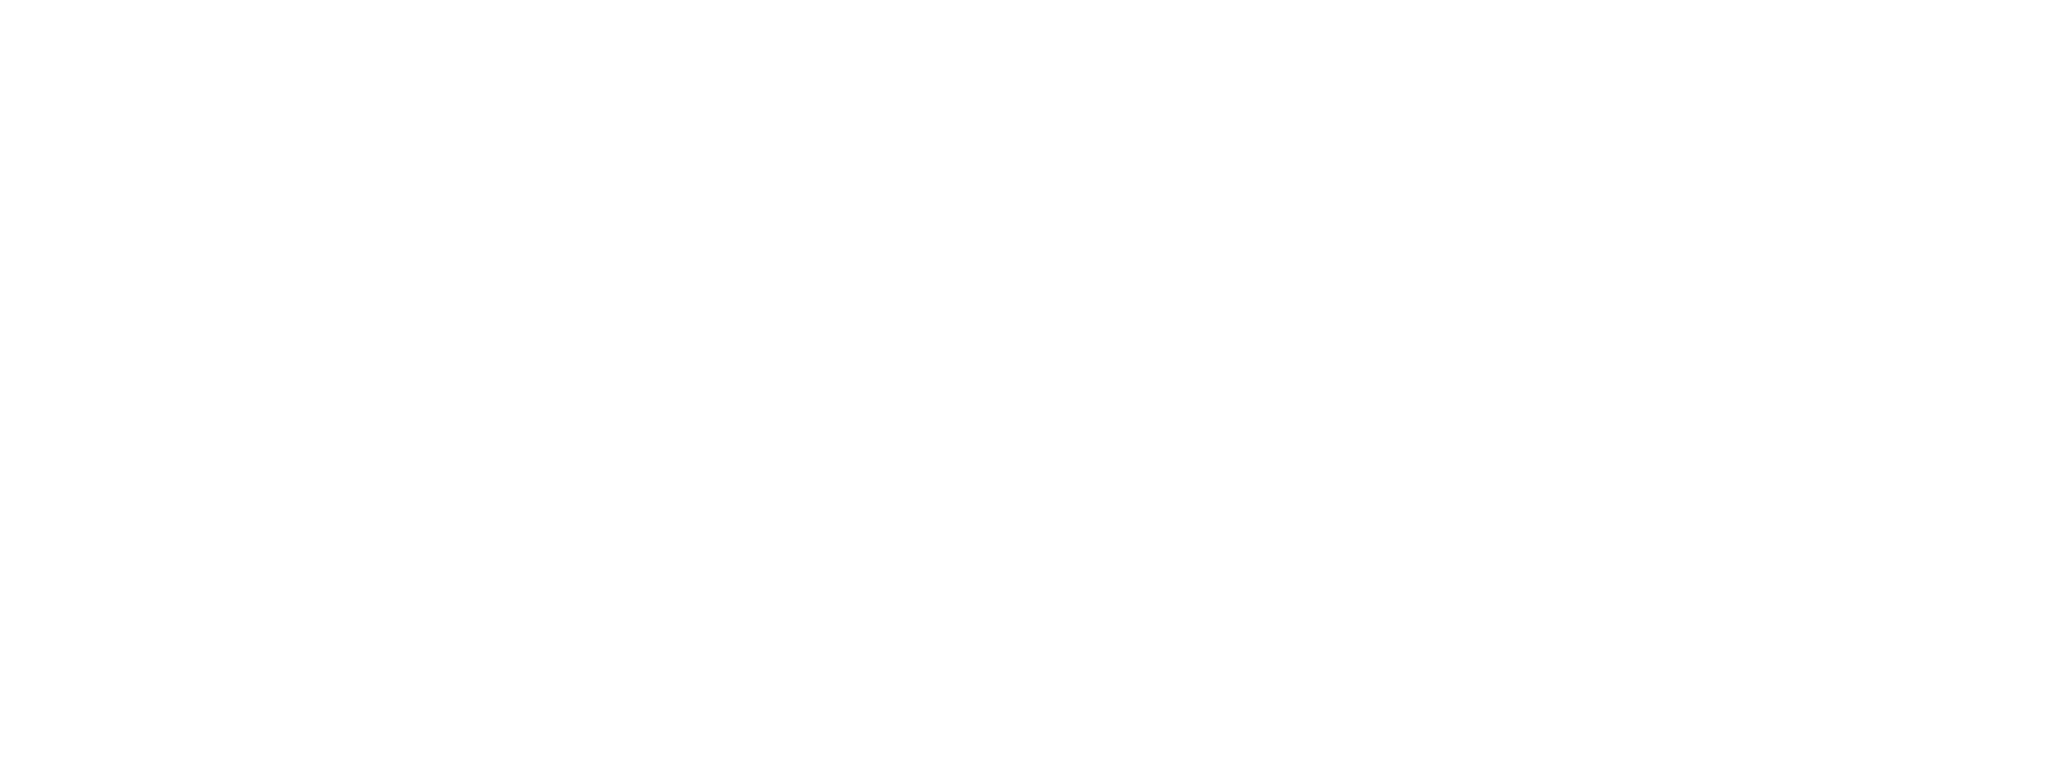
\includegraphics[width=0.5\textwidth]{cpu-vonNeumann.pdf}
\hfill
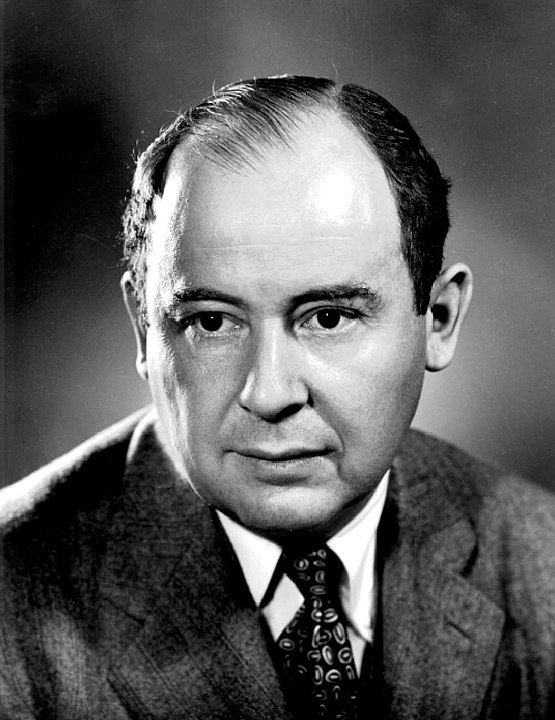
\includegraphics[width=0.2\textwidth]{fig/vonNeumann.png}
\end{center}
\begin{itemize}
\item 5 základních jednotek – řídicí jednotka, aritmeticko-logická jednotka, paměť, vstup (vstupní zařízení), výstup (výstupní zařízení)
\item Architektura počítače by neměla být závislá na řešené úloze, měla by umět provádět program uložený v paměti. Program řídí, co počítač vykonává za instrukce a tím jaké dostane výsledky.
\item Program a data jsou uložena ve stejné paměti, složené z buněk (jednotek) stejné velikosti. Oproti tomu Harvardská architektura měla jeden typ paměti pro program a jiný typ paměti pro data.
\item Další instrukce, která se bude vykonávat je uložena v následující buňce paměti (mimo skoků v programu)
\item Instrukce provádějí aritmetické a logické operace, přesuny dat z/do paměti, skoky a větvení programu a speciální řídicí instrukce.
\end{itemize}
\end{frame}


\begin{frame}
\frametitle{Počítač založený na von Neumannově konceptu}

Procesor / mikroprocesor:
\begin{itemize}
\item Řídicí jednota (control unit)
\item Aritmeticko-logická jednotka -- ALU
\end{itemize}

Paměť: 
\begin{itemize}
\item von Neumann architektura má společnou paměť pro program i data
\item paměť se skládá z buněk - jednotek, v současné době z bajtů
\end{itemize}

Vstupně výstupní podsystém:
\begin{itemize}
\item Vstupy -- klávesnice, myši, děrné štítky, magnetopáskové jednotky, síťové karty, ...
\item Výstupy -- monitory, tiskárny, plotry, síťové karty, ...
\end{itemize}

Řídicí jednotka řídí práci a sekvenci této práce. Skládá se z:
\begin{itemize}
\item registrů – udržují mezivýpočty a stavy výpočtů
\item řídicích hradel -- dekódují instrukce a provádí operace
\end{itemize}
\end{frame}


\begin{frame}
\frametitle{The most important registers of the control unit}
\begin{itemize}
\item PC (Program Counter)
holds address of a recent or next instruction to be processed
\item IR (Instruction Register)
holds the machine instruction read from memory
\item Another usually present registers
\begin{itemize}
\item General purpose registers (GPRs)
may be divided to address and data or (partially) specialized registers
\item SP (Stack Pointer) – points to the top of the stack; (The stack is usually used to store local variables and subroutine return addresses)
\item PSW (Program Status Word)
\item IM (Interrupt Mask)
\item Optional Floating point (FPRs) and vector/multimedia regs.
\end{itemize}
\end{itemize}
\end{frame}

\begin{frame}
\frametitle{The main instruction cycle of the CPU}
FLAGS registr 
\begin{enumerate}
  \item Initial setup/reset – set initial PC value, PSW, etc.
  \item Read the instruction from the memory
  \begin{itemize}
    \item PC → to the address bus
    \item Read the memory contents (machine instruction) and transfer it to the IR
    \item PC+l → PC, where l is length of the instruction
  \end{itemize}
  \item Decode operation code (opcode)
  \item Execute the operation
  \begin{itemize}
    \item compute effective address, select registers, read operands, pass them  through ALU and store result
  \end{itemize}
  \item Check for exceptions/interrupts (and service them)
  \item Repeat from the step 2
\end{enumerate}
\end{frame}


\begin{frame}[fragile,shrink=10]
\frametitle{Compilation: C  Assembler  Machine Code}

\begin{columns}
\begin{column}{0.3\textwidth}
\begin{lstlisting}[language={C},columns=flexible]
/* ffs as log2(x)*/
int x = 157;
int y = -1;
 
while(x != 0) {
  x = x / 2;
  y = y + 1;
}
\end{lstlisting}
\end{column}

\begin{column}{0.4\textwidth}  
\begin{lstlisting}[language={C},columns=flexible]
_start:
    // int x = 157;
  addi a0, zero, 157  
    // int y = 0;
  addi t1, zero, -1   
    // while(x != 0) {
  beq a0, zero, done  
loop:
    //   x = x / 2;
  srli a0, a0, 1 
    //   y = y + 1;
  addi t1, t1, 1      
    // }
  bne a0, zero, loop  
done:
\end{lstlisting}
\end{column}

\begin{column}{0.3\textwidth}  
\texttt{0x00000200  09d00513\\
0x00000204  fff00313\\
0x00000208  00050863\\
0x0000020c  00155513\\
0x00000210  00130313\\
0x00000214  fe051ce3\\
0x00000218  00030513\\
0x0000021c  00100073}
\end{column}

\end{columns}

\end{frame}


\begin{frame}
\frametitle{Instruction Encoding Constrains}
\begin{itemize}
\item Encode 256 combinations in 8-bits
\item Opcode and address to directly operate on megabytes of ram does not fit
\item Use some limited number of fast accessible registers or use stack concept
\item 8 registers, 3 bits to encode, for two operand operations (a += b, mem[a] = b), 6 bits to select registers→only 4 operations in total
\item 16 bit (65536), 16 registers, 256 two operands or 16 three operands (4 + 3 * 4 bits)
\item 32 bit, 32 registers, three operands (17 + 3 * 5)
\item But immediate for arithmetic and address usually required (CISC followup words, RISC uses limited ranges and some other mechanism) 
\end{itemize}
\end{frame}


\begin{frame}[shrink=5]
\frametitle{RISC-V -- Instruction Length Encoding}

\begin{tabular}{r l}
  \begin{tabular}{|c|}\hline
  \texttt{xxxxxxxxxxxxxxaa}\\ \hline
  \end{tabular} & 16-bit ($aa \neq 11$)\\
   &  \\
   \begin{tabular}{|c|c|}\hline
  \texttt{xxxxxxxxxxxxxxxx} & \texttt{xxxxxxxxxxxbbb11}\\ \hline
  \end{tabular} & 32-bit ($bbb \neq 111$)\\
 &  \\
   \begin{tabular}{c|c|c|}\hline
  \texttt{...xxxx} &\texttt{xxxxxxxxxxxxxxxx} & \texttt{xxxxxxxxxx011111}\\ \hline
  \end{tabular} & 48-bit\\
 &  \\
   \begin{tabular}{c|c|c|}\hline
  \texttt{...xxxx} &\texttt{xxxxxxxxxxxxxxxx} & \texttt{xxxxxxxxx0111111}\\ \hline
  \end{tabular} & 64-bit\\
 &  \\
   \begin{tabular}{c|c|c|}\hline
  \texttt{...xxxx} &\texttt{xxxxxxxxxxxxxxxx} & \texttt{xnnnxxxxx0111111}\\ \hline
  \end{tabular} & ($80+16\cdot nnn$)-bit\\
  & ($nnn \neq 111$)\\
   \begin{tabular}{c|c|c|}\hline
  \texttt{...xxxx} &\texttt{xxxxxxxxxxxxxxxx} & \texttt{x111xxxxx0111111}\\ \hline
  \end{tabular} & rezervováno pro\\
  & $\ge 192$-bit\\
Address: \phantom{\texttt{yyyyyxxxxxxxxxxxxxxxx    xxxxxxxxx0111111}}&  \\
base+4 \phantom{\texttt{xxxxxxx}} base+2 \phantom{\texttt{xxxxxxxxxxx}} base \phantom{\texttt{xxxxxxx}} &  \\
\end{tabular}

\end{frame}


\begin{frame}
\frametitle{RISC-V Processor Registers}
\begin{tabular}{l l l l}
Register & ABI Name & Description & Saver \\
x0 & zero & Hard-wired zero &  \\
x1 & ra & Return address & Caller \\
x2 & sp & Stack pointer &  Callee\\
x3 & gp & Global pointer &  \\
x4 & tp & Thread pointer &  \\
x5-7 & t0--2 & Temporaries &  \\
x8 & s0/fp & Saved register/frame pointer & Callee \\
x9 & s1 & Saved register &  Callee \\
x10--11 & a0--2 & Function arguments/return values &  Caller \\
x12--17 & a2--7 & Function arguments & Caller \\
x18--27 & s2--11 & Saved registers & Callee \\
x28--31 & t3--6 & Temporaries &  \\
pc & pc & Program Counter &  \\
f0-31 &  & Floating point &  \\
\end{tabular}
\end{frame}



\begin{frame}
\frametitle{Hardwarová realizace základního cyklu CPU}

\begin{center}
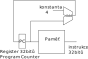
\includegraphics[width=0.75\textwidth]{cpu_step.pdf}
\end{center}

\end{frame}

\begin{frame}
\frametitle{Cíl přednášky}

\begin{itemize}
\item Porozumět implementaci jednoduchého počítače, který se skládá z
procesoru a oddělené paměti pro instrukce a data
\item Naším cílem je implementovat následující instrukce:
\item Číst a zapisovat hodnotu z/do datové paměti.
\begin{itemize}
\textbf{\texttt{lw}} - načtení slova, \textbf{\texttt{sw}} - uložení slova
\end{itemize}
\item aritmetické a logické instrukce: \textbf{\texttt{add}}, \textbf{\texttt{sub}}, \textbf{\texttt{and}}, \textbf{\texttt{or}}, \textbf{\texttt{slt}}
\begin{itemize}
\item Immediátové varianty: \textbf{\texttt{addi}}, \textbf{\texttt{ori}}, horní bity načítají \textbf{\texttt{olui}},\textbf{\texttt{auipc}}
\end{itemize}
\item Instrukce pro změnu toku programu/skok \textbf{\texttt{beq}}
\item Volání podprogramu \textbf{\texttt{jal}}, \textbf{\texttt{jalr}} (zajišťuje i návrat z podprogramu \textbf{\texttt{jr~ra}})
\item CPU se bude skládat z řídicí jednotky a ALU.
\item Poznámky:
\begin{itemize}
\item Implementace bude minimální (jednocyklový procesor - všechny operace budou probíhat v jednom cyklu, tzn.
zpracovány v jednom kroku/hodině)
\item Přednáška 5 je zaměřena na efektivnější realističtější implementaci zřetězenného (pipelined) CPU.
\end{itemize}
\end{itemize}

\end{frame}


\begin{frame}
\frametitle{Instrukce RISC-V implementované v této přednášce}


\end{frame}


\begin{frame}
\frametitle{Základní stavební bloky CPU}


\end{frame}


\begin{frame}
\frametitle{Instrukce lw -- load word}

\textbf{\texttt{lw -- load word}} načti slovo z paměti do registru

\begin{tabular}{|l|l|}\hline
Popis & Načte slovo do registru ze zadané adresy z paměti \\ \hline
Operace & \texttt{[rd]} $\leftarrow$ \texttt{Mem[[rs]+imm12]} \\ \hline
Syntax & lw rd, imm12(rs) \\ \hline
Kódování & \texttt{iiii iiii iiii ssss s010 dddd d000 0011} \\ \hline
\end{tabular}

Příklad: Načtěte 32-bitové slovo z paměti z adresy 0x400 do registru 2:\\
\textbf{\texttt{lw x2, 0x400(x0)}}

\textbf{\texttt{iiii iiii iiii}}\phantom{xx}\textbf{\texttt{ssss s}}\hspace{0.1cm}\textbf{\texttt{010\hspace{0.25cm}dddd d\hspace{0.05cm}000 0011}}\\
\underbrace{\textbf{\texttt{0100 0000 0000}}}_{0x400}\texttt{ }\underbrace{\textbf{\texttt{0000 0}}}_{0}\underbrace{\textbf{\texttt{010}}}_{func3}\phantom{i}\underbrace{\textbf{\texttt{0001 0}}}_{2}\underbrace{\textbf{\texttt{000 0011}}}_{opcode}\\

\textbf{\texttt{0x 40 00 21 03}} -- kód pro instrukci \textbf{\texttt{lw x2, 0x400(x0)}}

Poznámka: Registr x0 má natvrdo hodnotu 0, kterou nelze změnit

\end{frame}

\begin{frame}[shrink=15]
\frametitle{Implementace instrukce lw}

\textbf{\texttt{lw}}: \texttt{rs1} -- základní adresa, \texttt{imm12} -- posunutí adresy, \texttt{rd} -- registr, kam se uloží data z paměti

\bigskip

\begin{tabular}{|l|l|l|l|l|l|}\hline
I & \textbf{\texttt{imm(12)}}, 31:20 & \textbf{\texttt{rs1(5)}}, 19:15 & \textbf{\texttt{func3}}, 14:12 & \textbf{\texttt{rd(5)}}, 11:7 & \textbf{\texttt{opcode(7)}}, 6:0 \\ \hline
\end{tabular}

\bigskip

\begin{center}
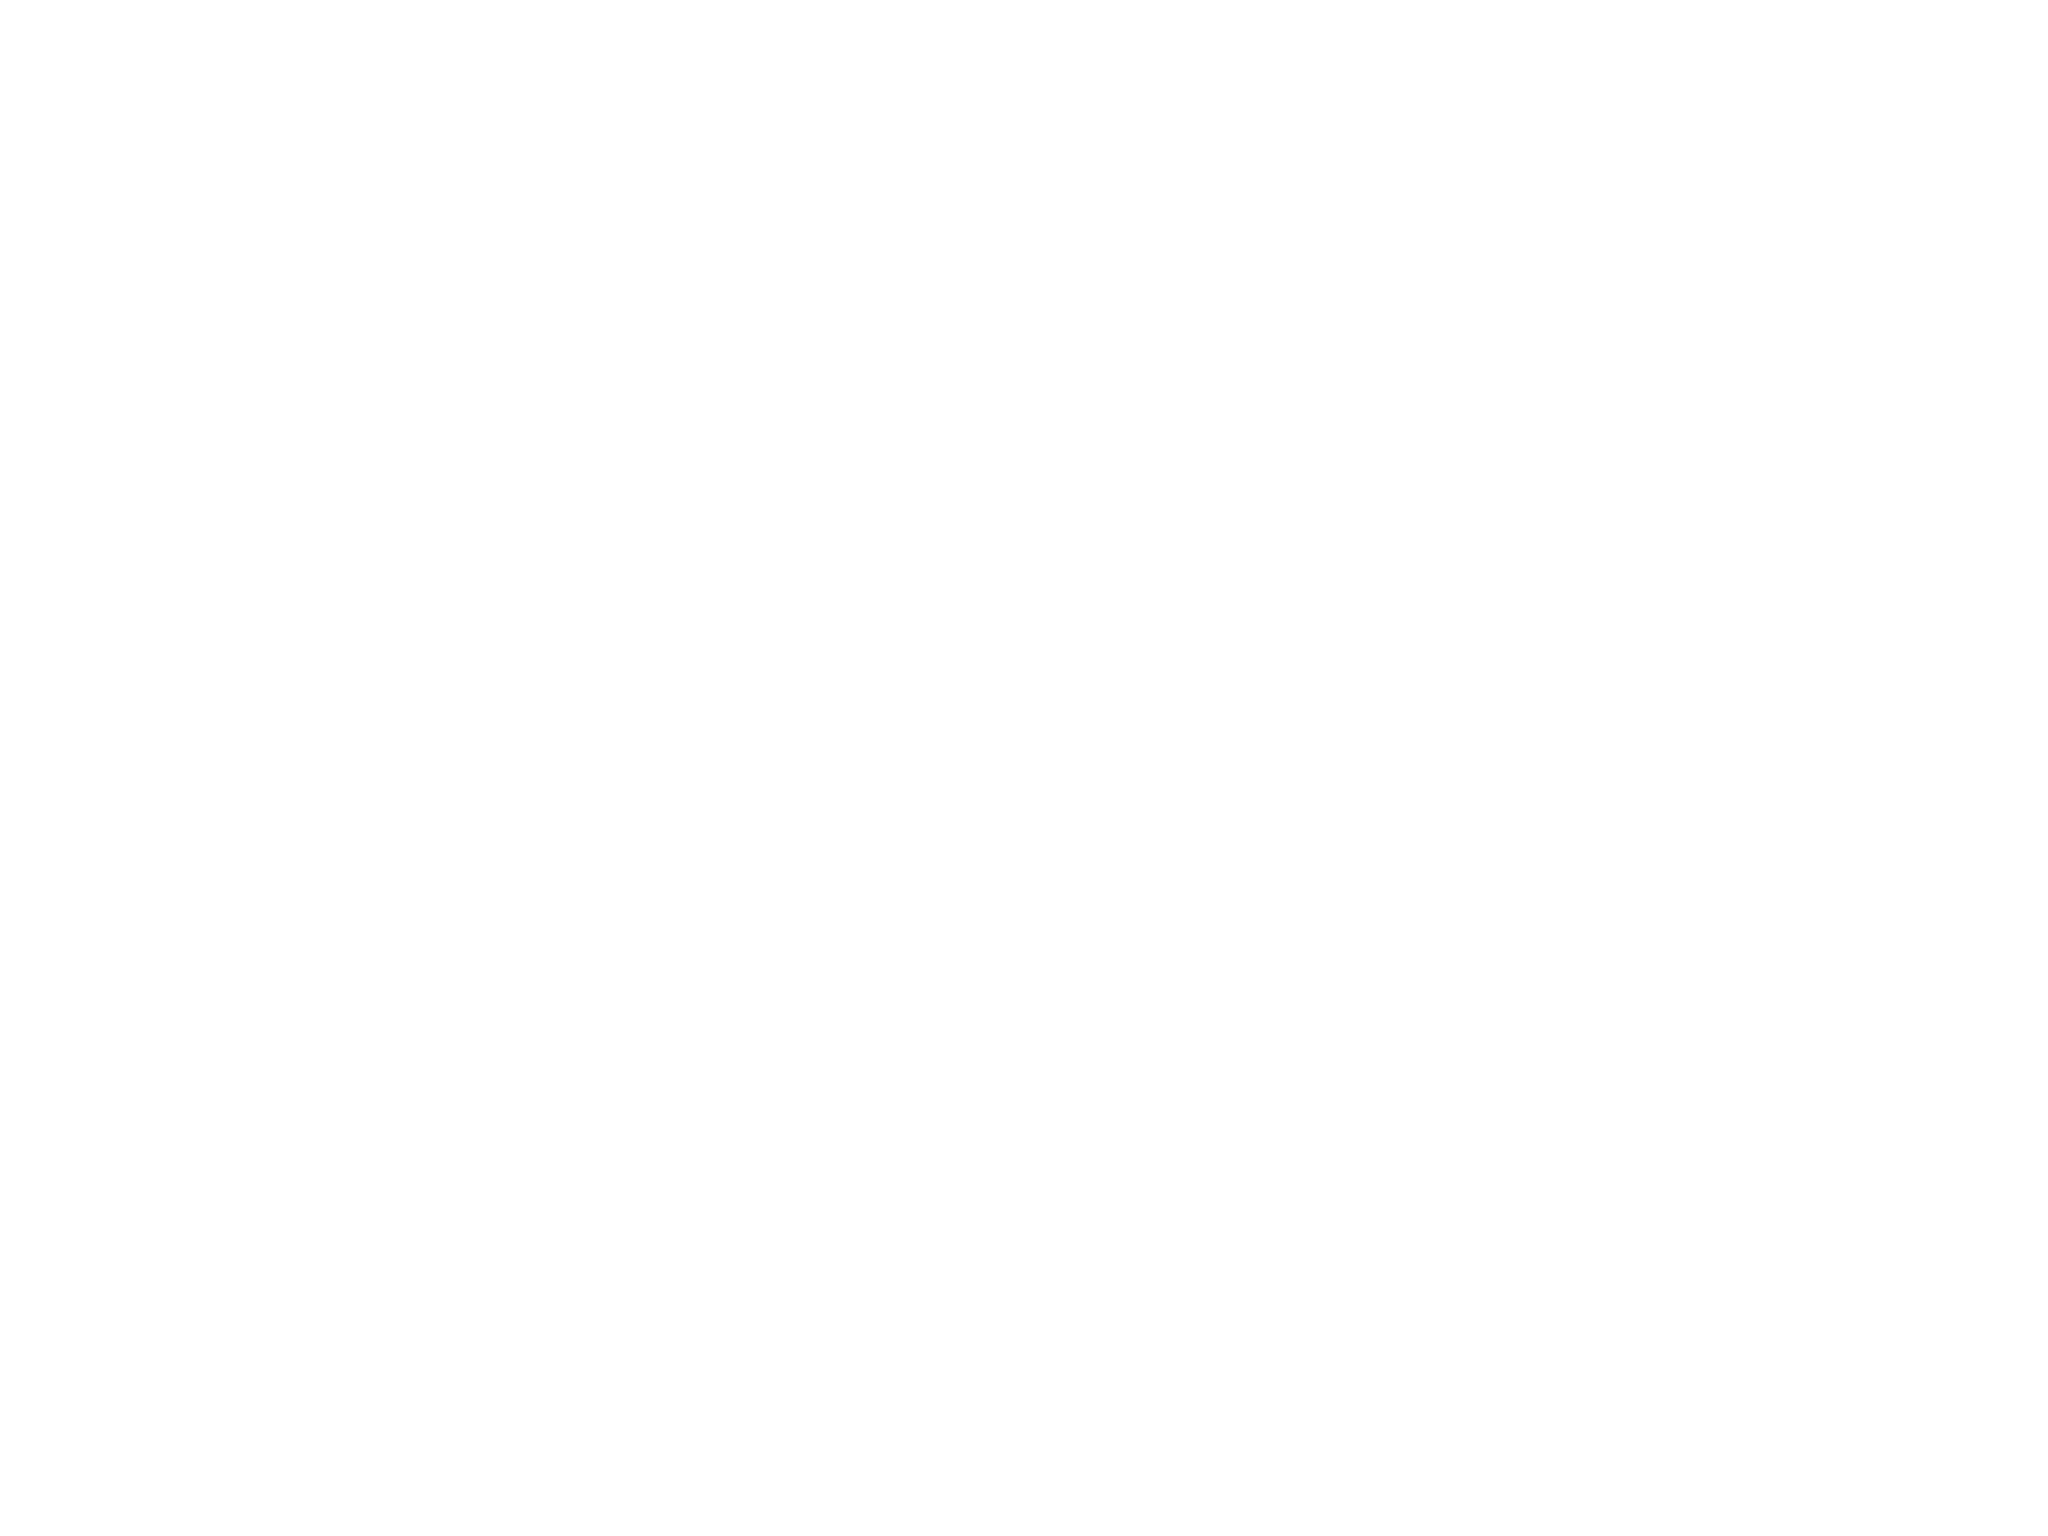
\includegraphics[width=0.90\textwidth]{cpu-load.pdf}
\end{center}

\end{frame}

\begin{frame}[shrink=15]
\frametitle{Implementace instrukce lw}

\textbf{\texttt{lw}}: \texttt{rs1} -- základní adresa, \texttt{imm12} -- posunutí adresy, \texttt{rd} -- registr, kam se uloží data z paměti

\bigskip

\begin{tabular}{|l|l|l|l|l|l|}\hline
I & \textbf{\texttt{imm(12)}}, 31:20 & \textbf{\texttt{rs1(5)}}, 19:15 & \textbf{\texttt{func3}}, 14:12 & \textbf{\texttt{rd(5)}}, 11:7 & \textbf{\texttt{opcode(7)}}, 6:0 \\ \hline
\end{tabular}

Zápis proběhna na rostoucí hranu hodin.

\begin{center}
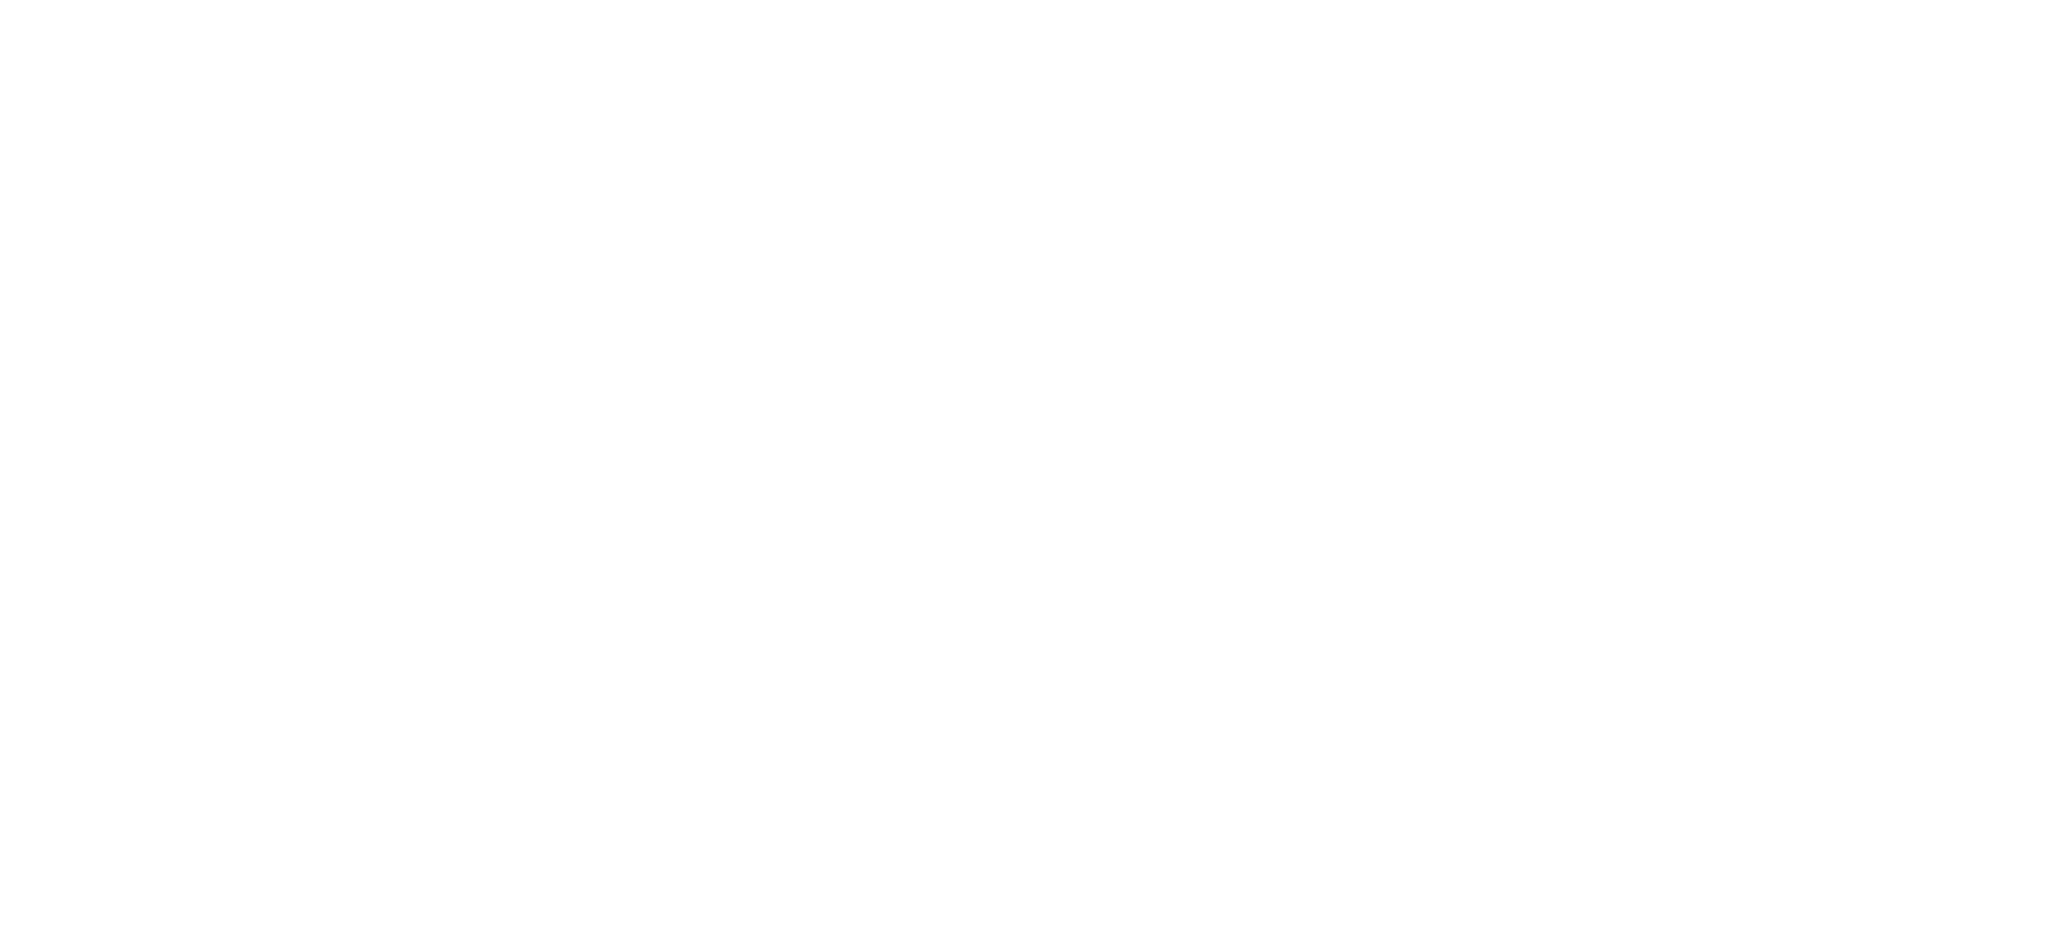
\includegraphics[width=0.90\textwidth]{cpu-load-red.pdf}
\end{center}



\end{frame}


\begin{frame}[shrink=15]
\frametitle{Implementace instrukce lw}

\textbf{\texttt{lw}}: \texttt{rs1} -- základní adresa, \texttt{imm12} -- posunutí adresy, \texttt{rd} -- registr, kam se uloží data z paměti

\bigskip

\begin{tabular}{|l|l|l|l|l|l|}\hline
I & \textbf{\texttt{imm(12)}}, 31:20 & \textbf{\texttt{rs1(5)}}, 19:15 & \textbf{\texttt{func3}}, 14:12 & \textbf{\texttt{rd(5)}}, 11:7 & \textbf{\texttt{opcode(7)}}, 6:0 \\ \hline
\end{tabular}

\bigskip

\begin{center}
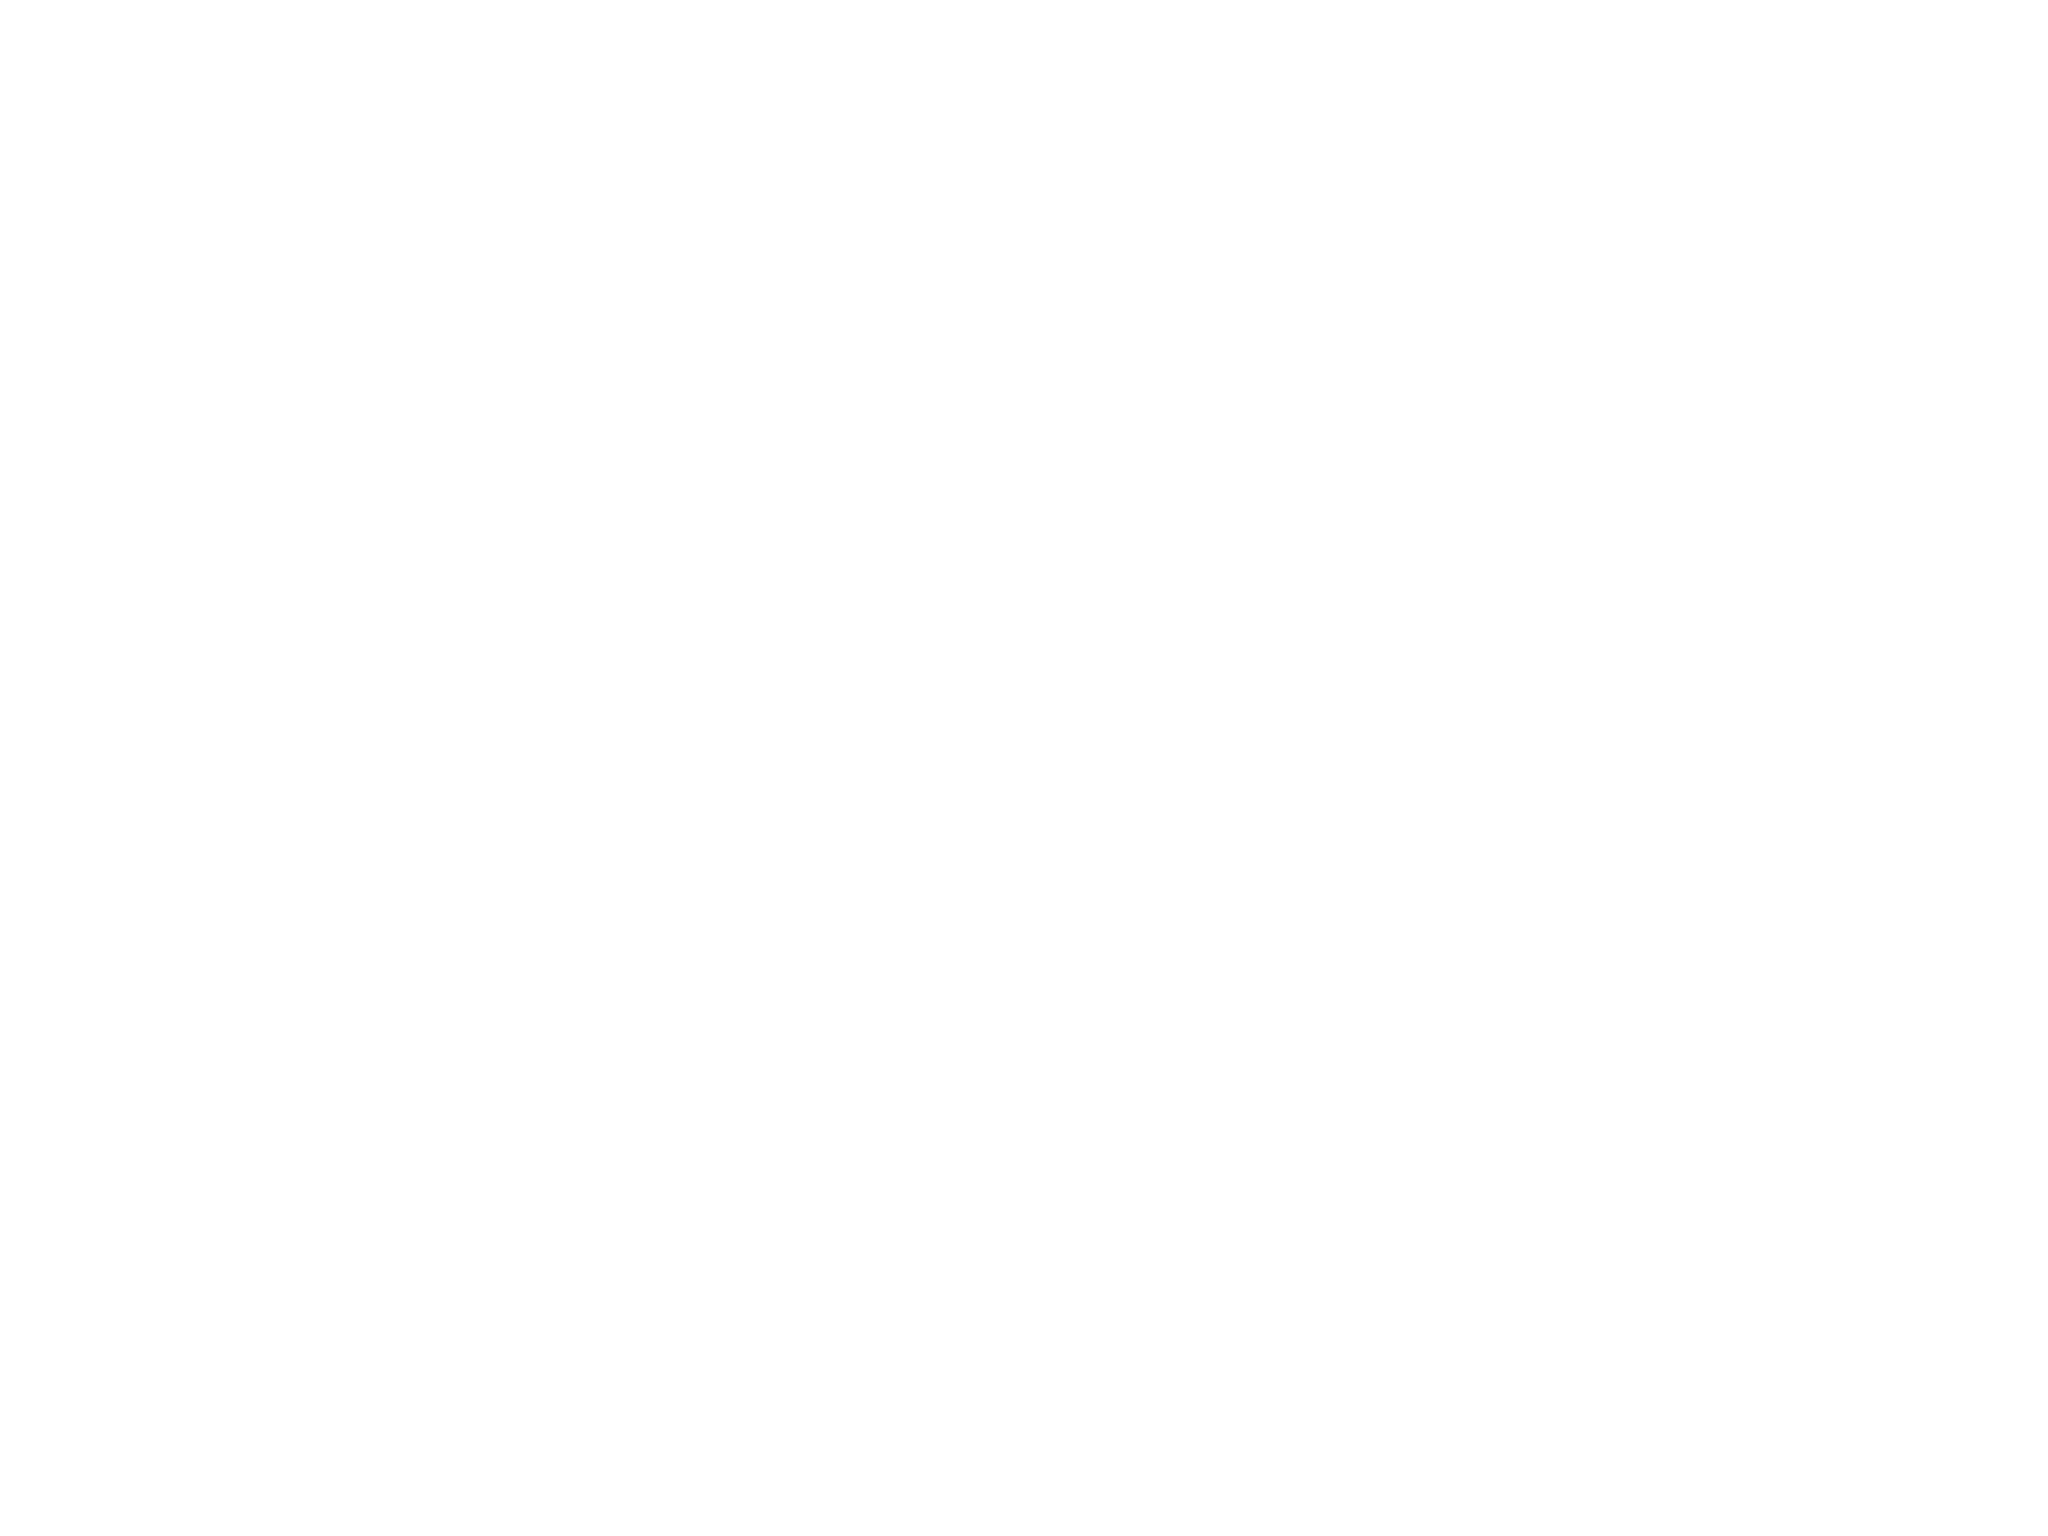
\includegraphics[width=0.88\textwidth]{cpu-load2.pdf}
\end{center}
\end{frame}


\begin{frame}
\frametitle{QtRvSim - RISC-V Simultaor}

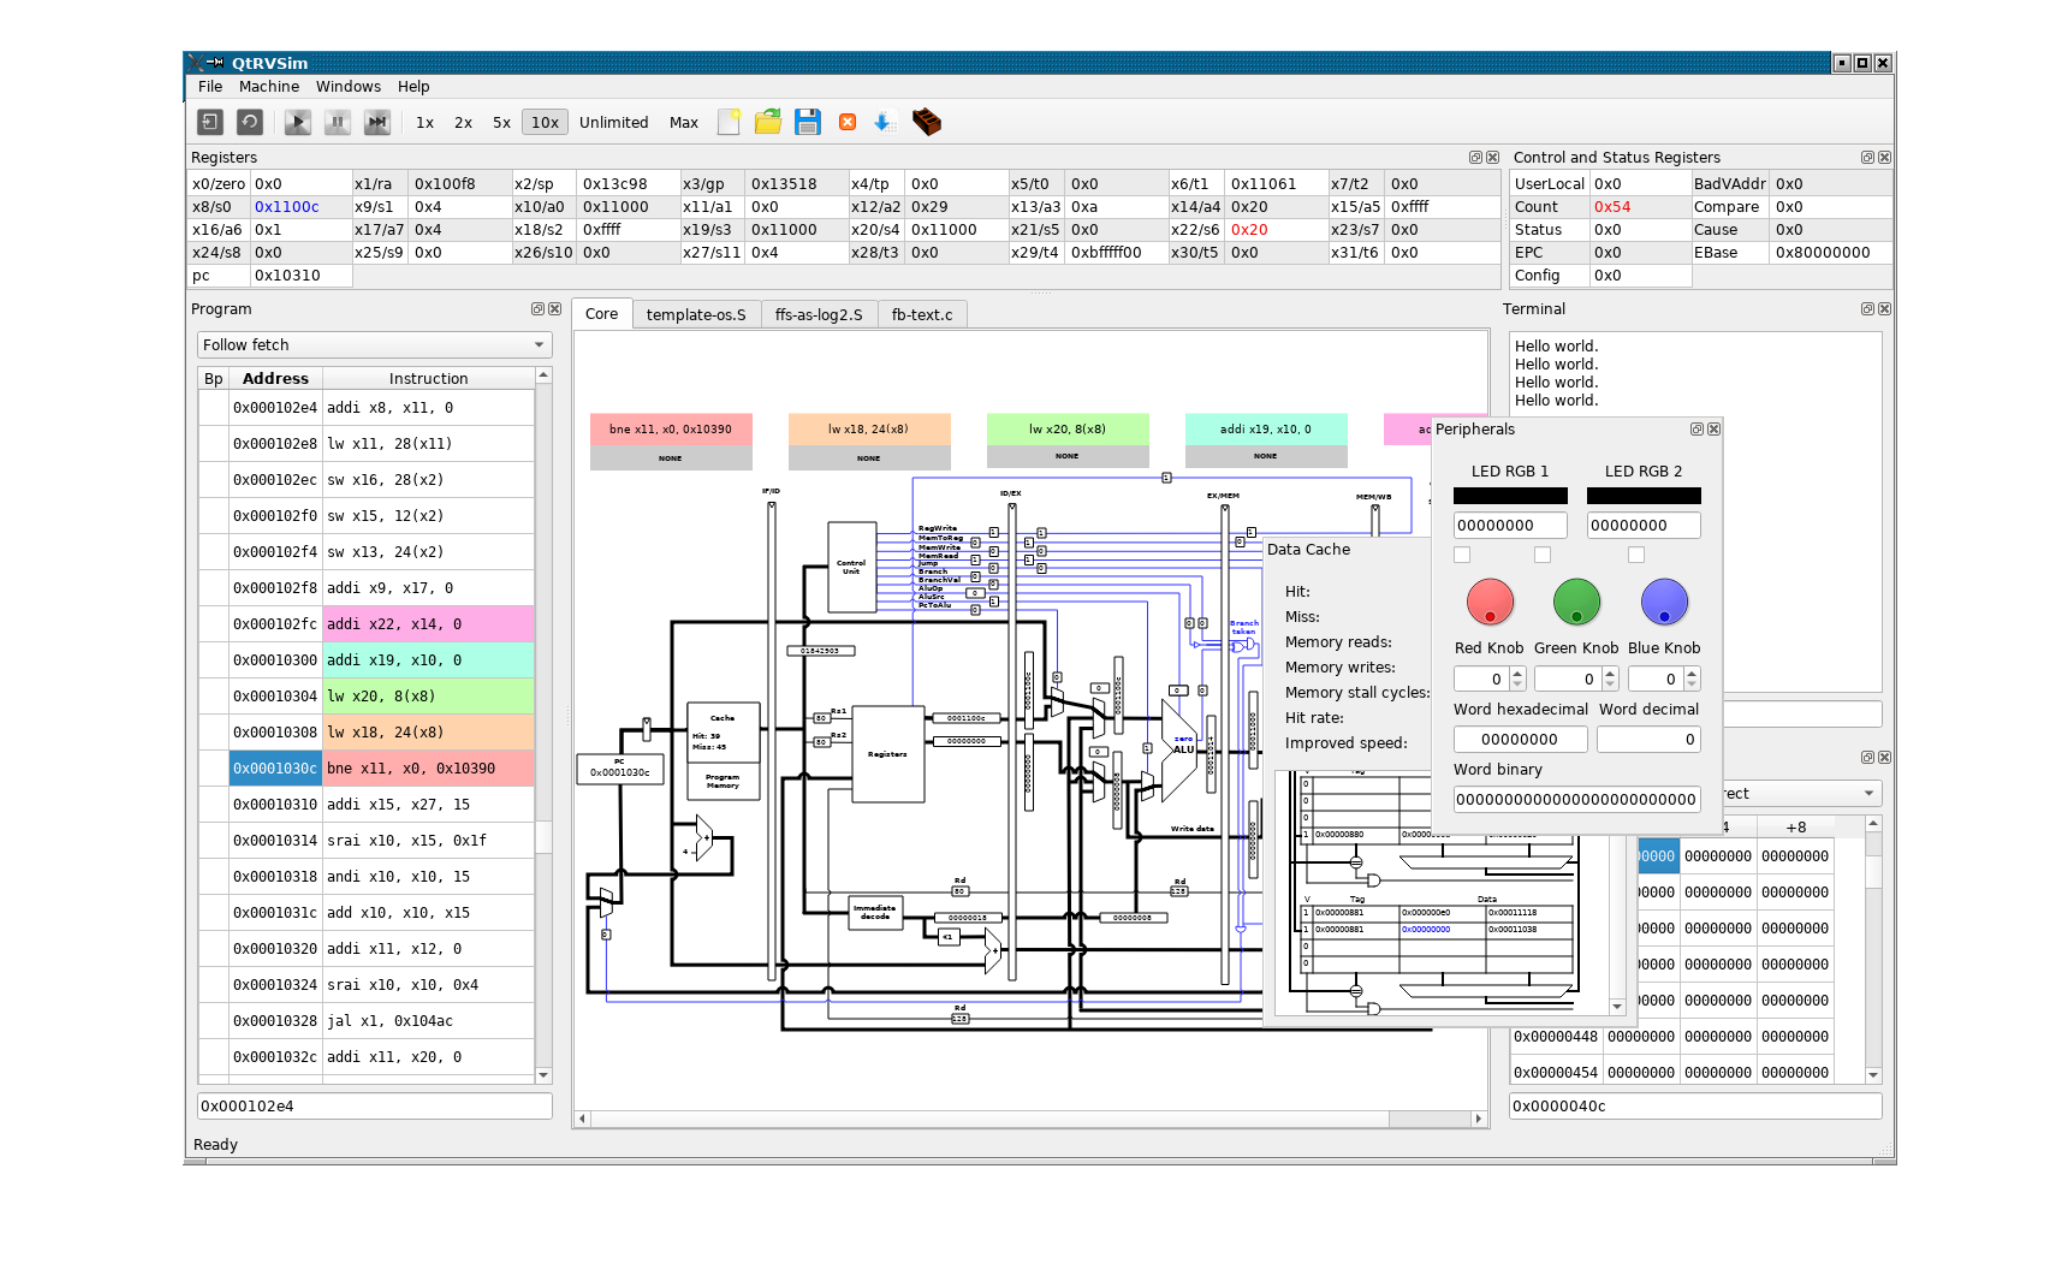
\includegraphics[width=0.9\textwidth]{simulator.pdf}

\end{frame}



\begin{frame}
\frametitle{Instrukce sw -- store word}

\textbf{\texttt{sw -- store word}} ulož slovo z registru do paměti

\bigskip

\begin{tabular}{|l|l|}\hline
Popis & Uloží slovo z registru rs2 do zadané adresy z paměti \\ \hline
Operace & \texttt{Mem[[rs1]+imm12]} $\leftarrow$ \texttt{[rs2]} \\ \hline
Syntax & sw rs2, imm12(rs1) \\ \hline
Kódování & \texttt{iiii iiit tttt ssss s010 iiii i010 0011} \\ \hline
\end{tabular}

\bigskip

Příklad: Načtěte 32-bitové slovo z paměti z adresy 0x400 do registru 2:\\
\textbf{\texttt{lw x2, 0x400(x0)}}

\textbf{\texttt{iiii iii\hspace{0.08cm}t tttt}}\phantom{xx}\textbf{\texttt{ssss s}}\hspace{0.1cm}\textbf{\texttt{010\hspace{0.25cm}dddd d\hspace{0.05cm}010 0011}}\\
\underbrace{\textbf{\texttt{0100 000}}}_{0x40\_}
\underbrace{\textbf{\texttt{0 0010}}}_{2}
\texttt{ }\underbrace{\textbf{\texttt{0010 1}}}_{5}
\underbrace{\textbf{\texttt{010}}}_{func3}\phantom{i}\underbrace{\textbf{\texttt{0010 0}}}_{0x \_04}
\underbrace{\textbf{\texttt{010 0011}}}_{opcode}\\

\textbf{\texttt{0x 40 22 a2 23}} -- kód pro instrukci \textbf{\texttt{sw x2, 0x404(x5)}}

\end{frame}

\begin{frame}[shrink=18]
\frametitle{Implementace instrukce sw}

\textbf{\texttt{sw}}: \texttt{rs1} -- základní adresa, \texttt{imm12} -- posunutí adresy, \texttt{rs2} -- registr, který se uloží do paměti

\bigskip

\begin{tabular}{|l|l|l|l|l|l|}\hline
S & \textbf{\texttt{imm(12)}},31:25,11:7 & \textbf{\texttt{rs2(5)}},24:20 & \textbf{\texttt{rs1(5)}},19:15 & \textbf{\texttt{func3}},14:12 & \textbf{\texttt{opcode(7)}},6:0 \\ \hline
\end{tabular}

\bigskip

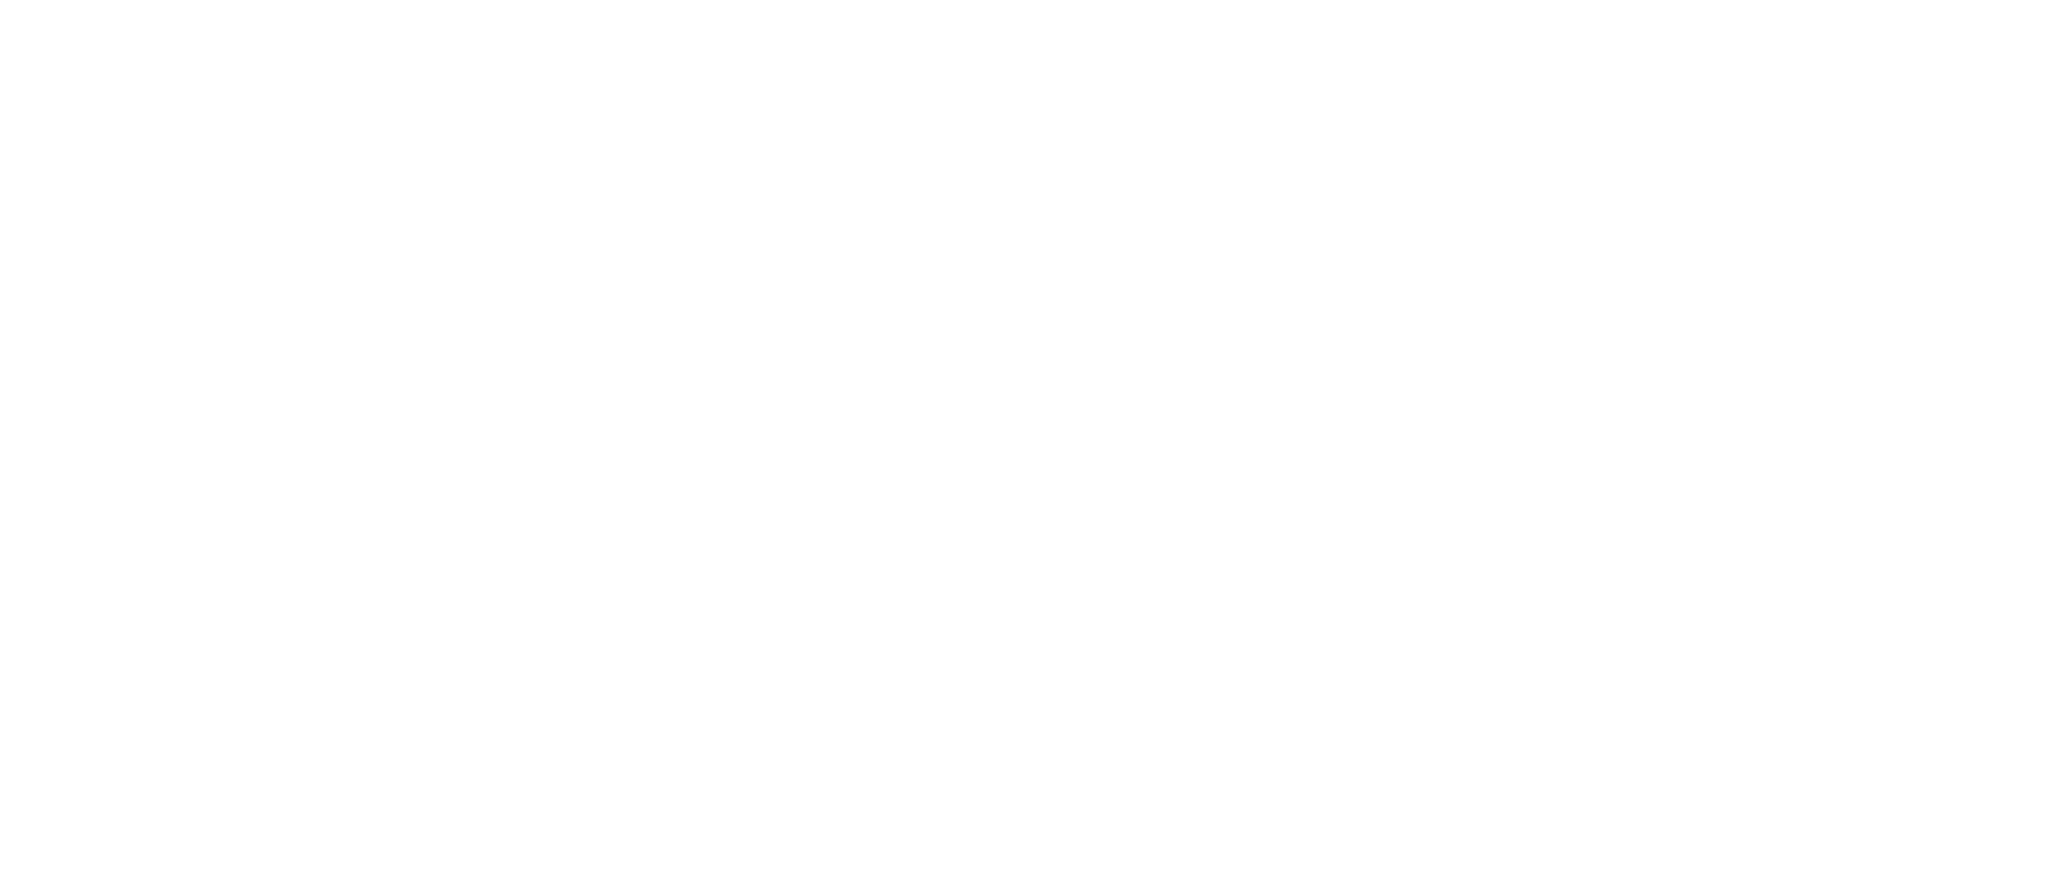
\includegraphics[width=0.90\textwidth]{cpu-store2.pdf}

\end{frame}




\begin{frame}
\frametitle{Instrukce add -- sečti dva registry}

\textbf{\texttt{add -- addition}} -- sečti hodnoty dvou registrů a součet ulož do registru

\bigskip

\begin{tabular}{|l|l|}\hline
Popis & Sečti hodnoty z registrů rs1 a rs2 a výsledek ulož do rd \\ \hline
Operace & \texttt{[rd]} $\leftarrow$ \texttt{[rs1] + [rs2]} \\ \hline
Syntax & add rd, rs1, rs2 \\ \hline
Kódování & \texttt{0000 000t tttt ssss s010 dddd d011 0011} \\ \hline
\end{tabular}

\bigskip

Příklad: Sečti hodnoty z registru 2 a registru 3, výsledek ulož do registru 4:\\
\textbf{\texttt{add x4, x2, x3}}

\textbf{\texttt{0000 000\hspace{0.08cm}t tttt}}\phantom{xx}\textbf{\texttt{ssss s}}\hspace{0.1cm}\textbf{\texttt{010\hspace{0.25cm}dddd d\hspace{0.05cm}010 0011}}\\
\textbf{\texttt{0000 000}}
\underbrace{\textbf{\texttt{0 0011}}}_{3}
\texttt{ }\underbrace{\textbf{\texttt{0001 0}}}_{2}
\underbrace{\textbf{\texttt{010}}}_{func3}\phantom{i}
\underbrace{\textbf{\texttt{0010 0}}}_{4}
\underbrace{\textbf{\texttt{011 0011}}}_{opcode}\\

\textbf{\texttt{0x 00 31 02 33}} -- kód pro instrukci \textbf{\texttt{add x4, x2, x3}}


\end{frame}

\begin{frame}[shrink=25]
\frametitle{Implementace instrukce add}

\textbf{\texttt{add}}: \texttt{rs1}, \texttt{rs2} -- sčítance, \texttt{rd} -- registr, kam se uloží součet

\bigskip

\begin{tabular}{|l|l|l|l|l|l|l|}\hline
R & \textbf{\texttt{func(7)}},31:25 & \textbf{\texttt{rs2(5)}},24:20 & \textbf{\texttt{rs1(5)}},19:15 & \textbf{\texttt{func3}},14:12 & \textbf{\texttt{rd(5)}},11:7 & \textbf{\texttt{opcode(7)}},6:0 \\ \hline
\end{tabular}

\bigskip

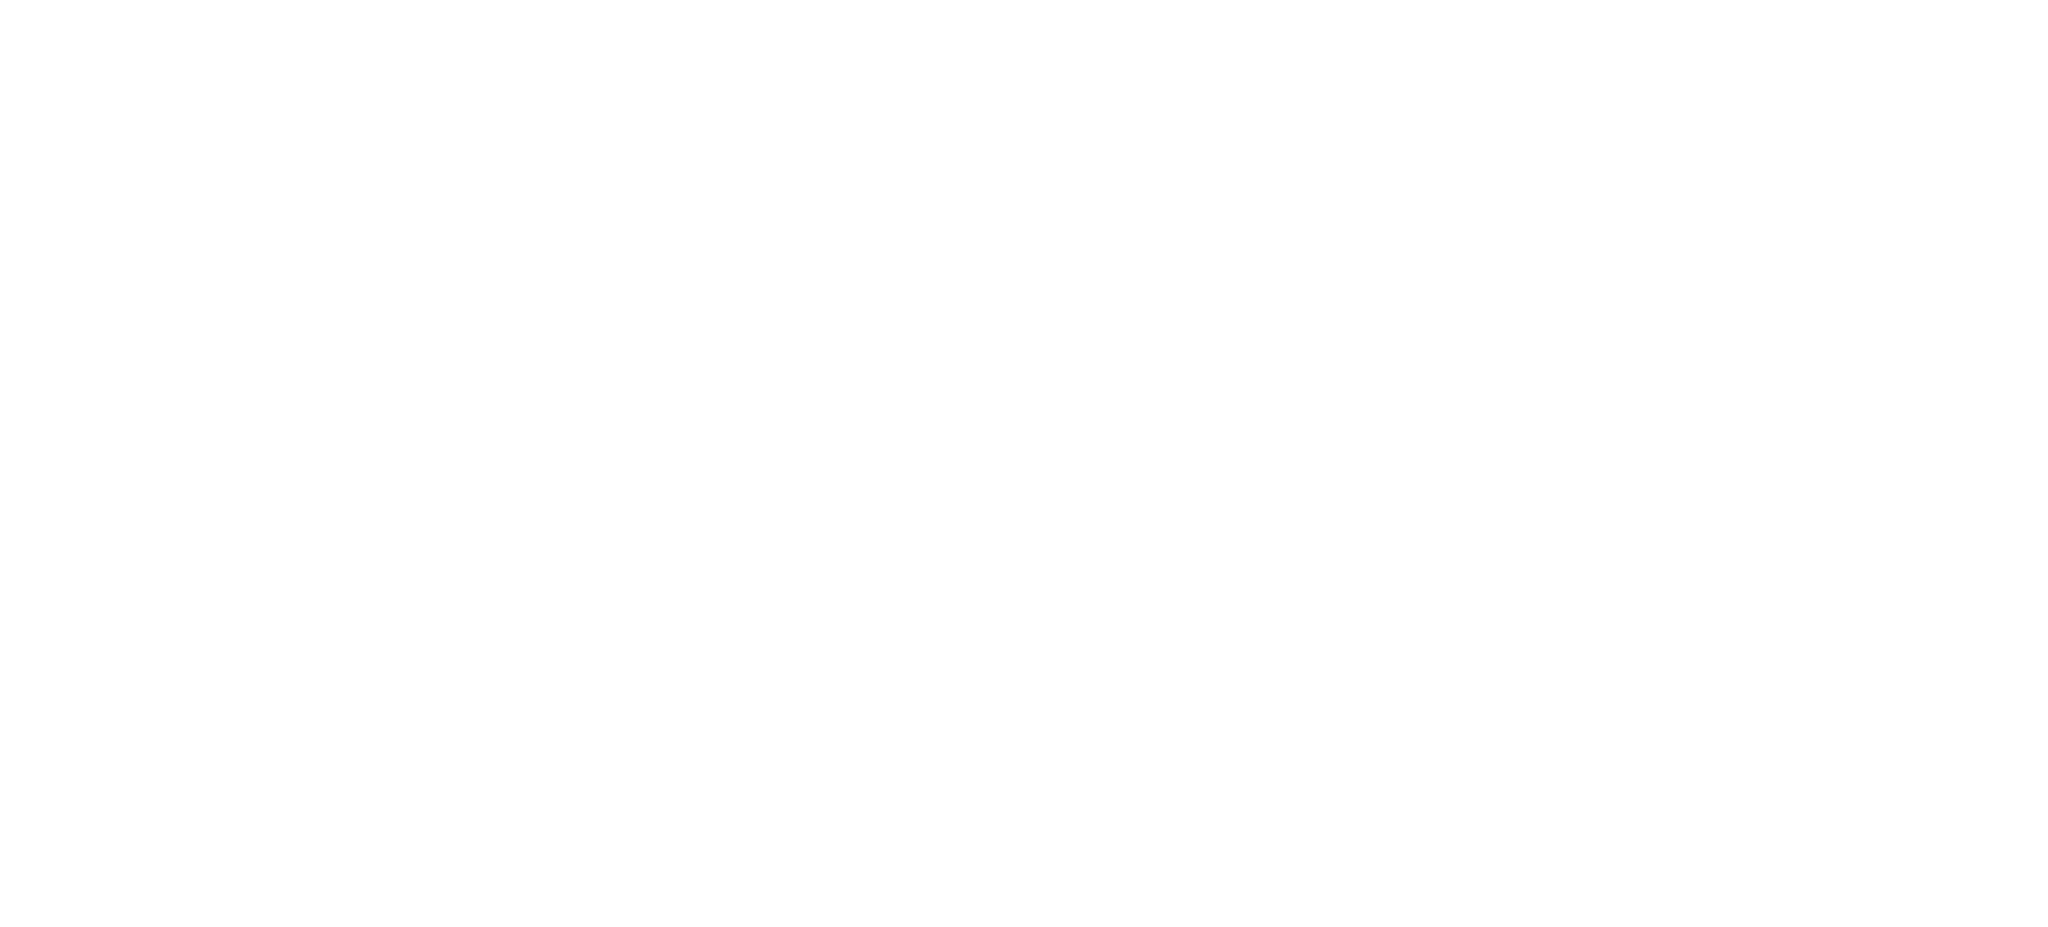
\includegraphics[width=0.85\textwidth]{cpu-add.pdf}

\end{frame}


\begin{frame}
\frametitle{Implementace instrukce sub, amd, or, slt}

Jediný rozdíl oproti instrukci sčítání add je v hodnotě ALUControl, který vybírá, jakou operaci jednotka ALU provede. Cesta dat a uložení výsledku je stejná jako u sčítání.
\bigskip

\bigskip

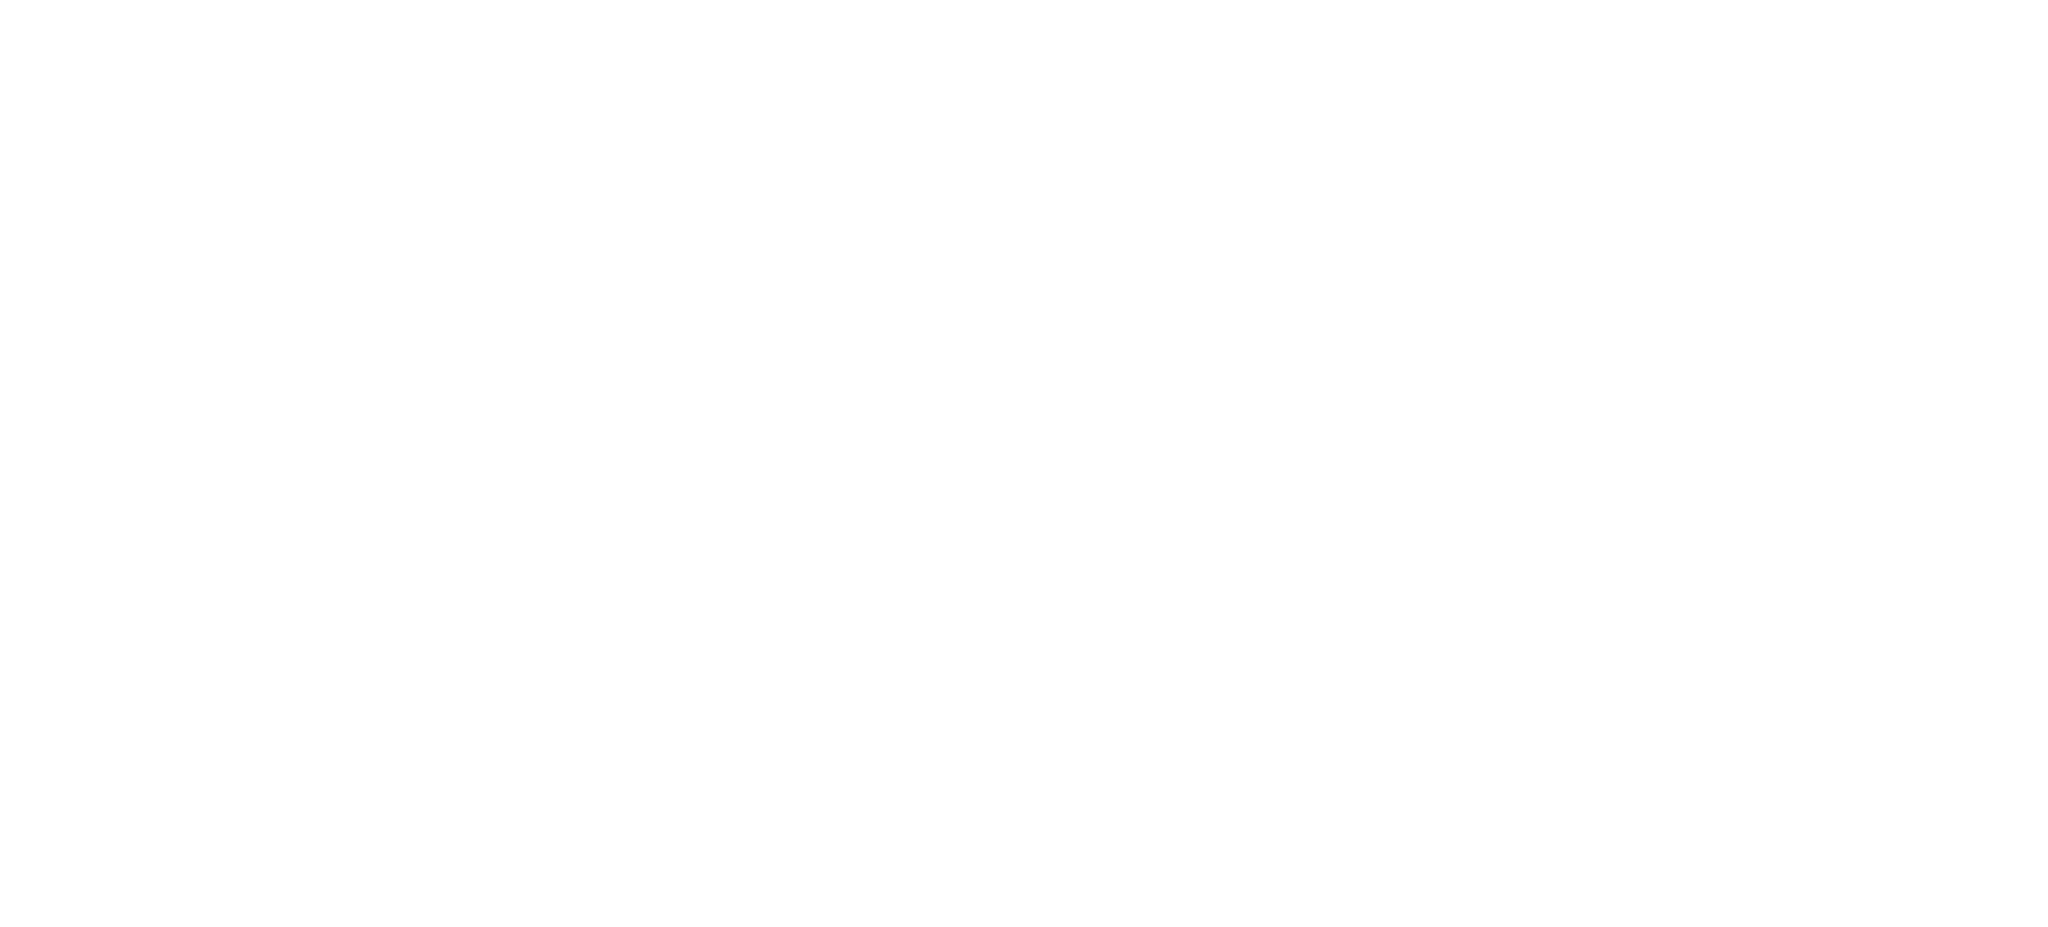
\includegraphics[width=0.85\textwidth]{cpu-add2.pdf}

\end{frame}


\begin{frame}[shrink=10]
\frametitle{Implementace instrukcí addi, ori, andi}

\textbf{\texttt{addi -- add immediate}}: \texttt{[rd]} $\leftarrow$ \texttt{[rs1] + imm12} -- přičte k hodnotě registru \texttt{rs1} konkrétní číslo \texttt{imm} a výsledek uloží do registru \texttt{rd}

\bigskip

\begin{tabular}{|l|l|l|l|l|l|}\hline
I & \textbf{\texttt{imm(12)}},31:20 & \textbf{\texttt{rs1(5)}},19:15 & \textbf{\texttt{func3}},14:12 & \textbf{\texttt{rd(5)}},11:7 & \textbf{\texttt{opcode(7)}},6:0 \\ \hline
\end{tabular}

\bigskip

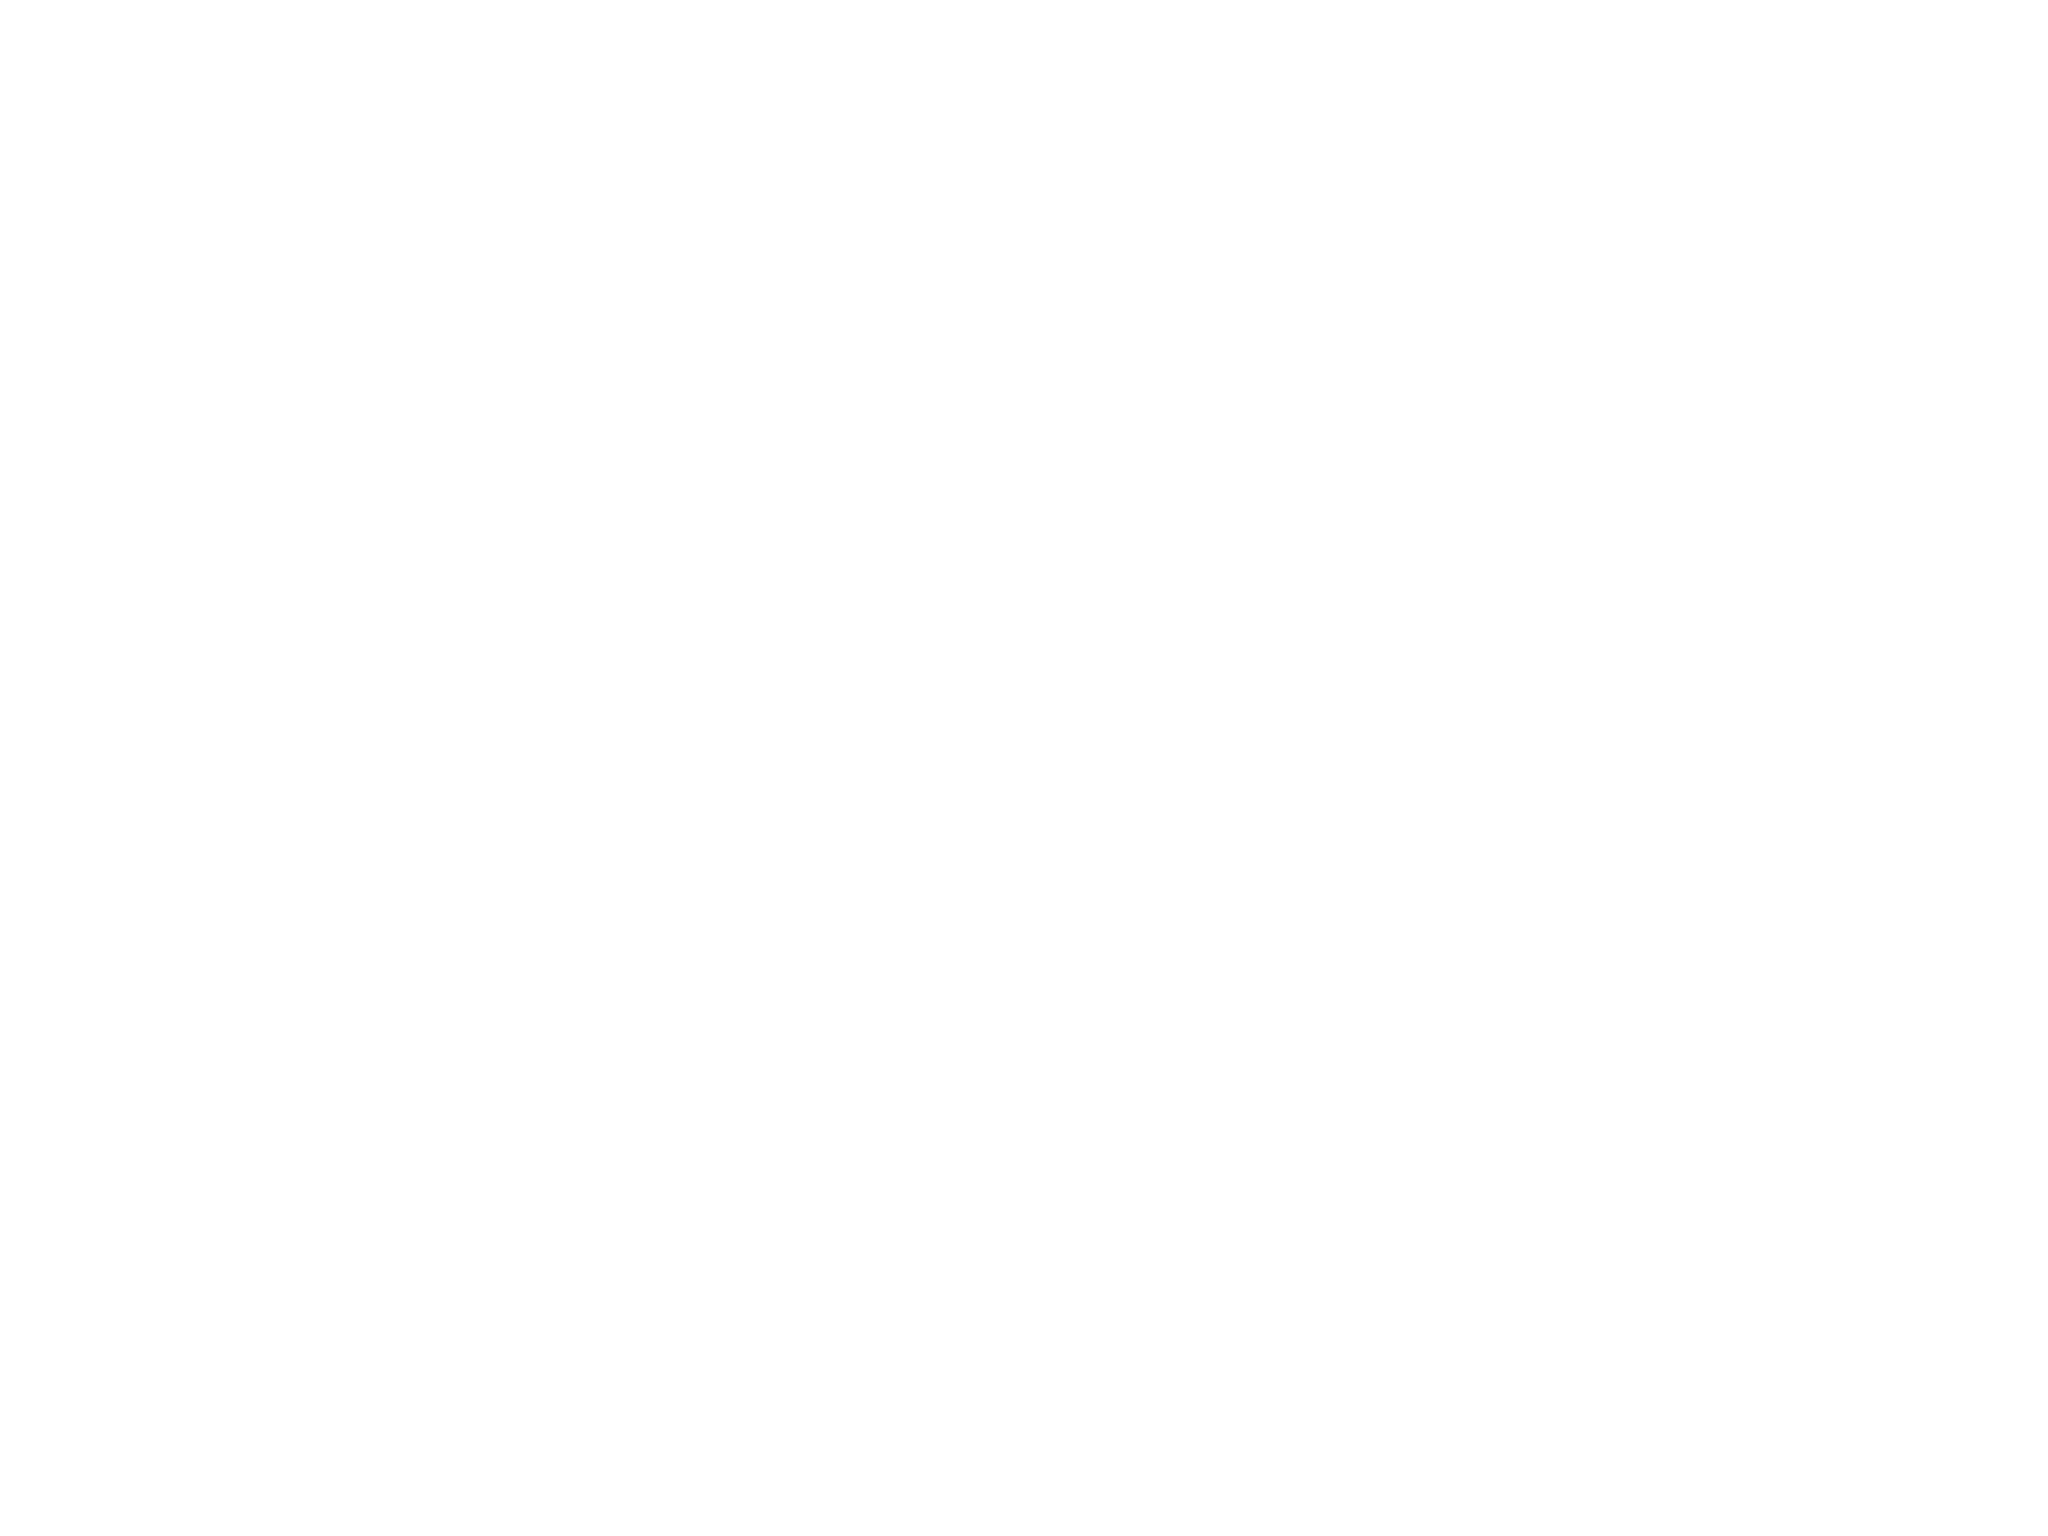
\includegraphics[width=0.85\textwidth]{cpu-addi.pdf}

\end{frame}


\begin{frame}[shrink=15]
\frametitle{Implementace instrukce skoku beq}

\textbf{\texttt{beq -- branch if equal}}: \texttt{[pc]} $\leftarrow$ \texttt{[pc] + SignImm} -- přičte k hodnotě registru \texttt{pc} konkrétní znaménkové číslo rozšířené na 32 bitů \texttt{imm} a výsledek uloží do registru \texttt{pc} pokud nastala rovnost hodnot v registrech rs1 a rs2.

\bigskip

\begin{tabular}{|l|l|l|l|l|l|}\hline
S & \textbf{\texttt{imm(12)}},31:25, 11:7 & \textbf{\texttt{rs2(5)}},24:20 & \textbf{\texttt{rs1(5)}},19:15 & \textbf{\texttt{func3}},14:12 & \textbf{\texttt{opcode(7)}},6:0 \\ \hline
\end{tabular}

\bigskip

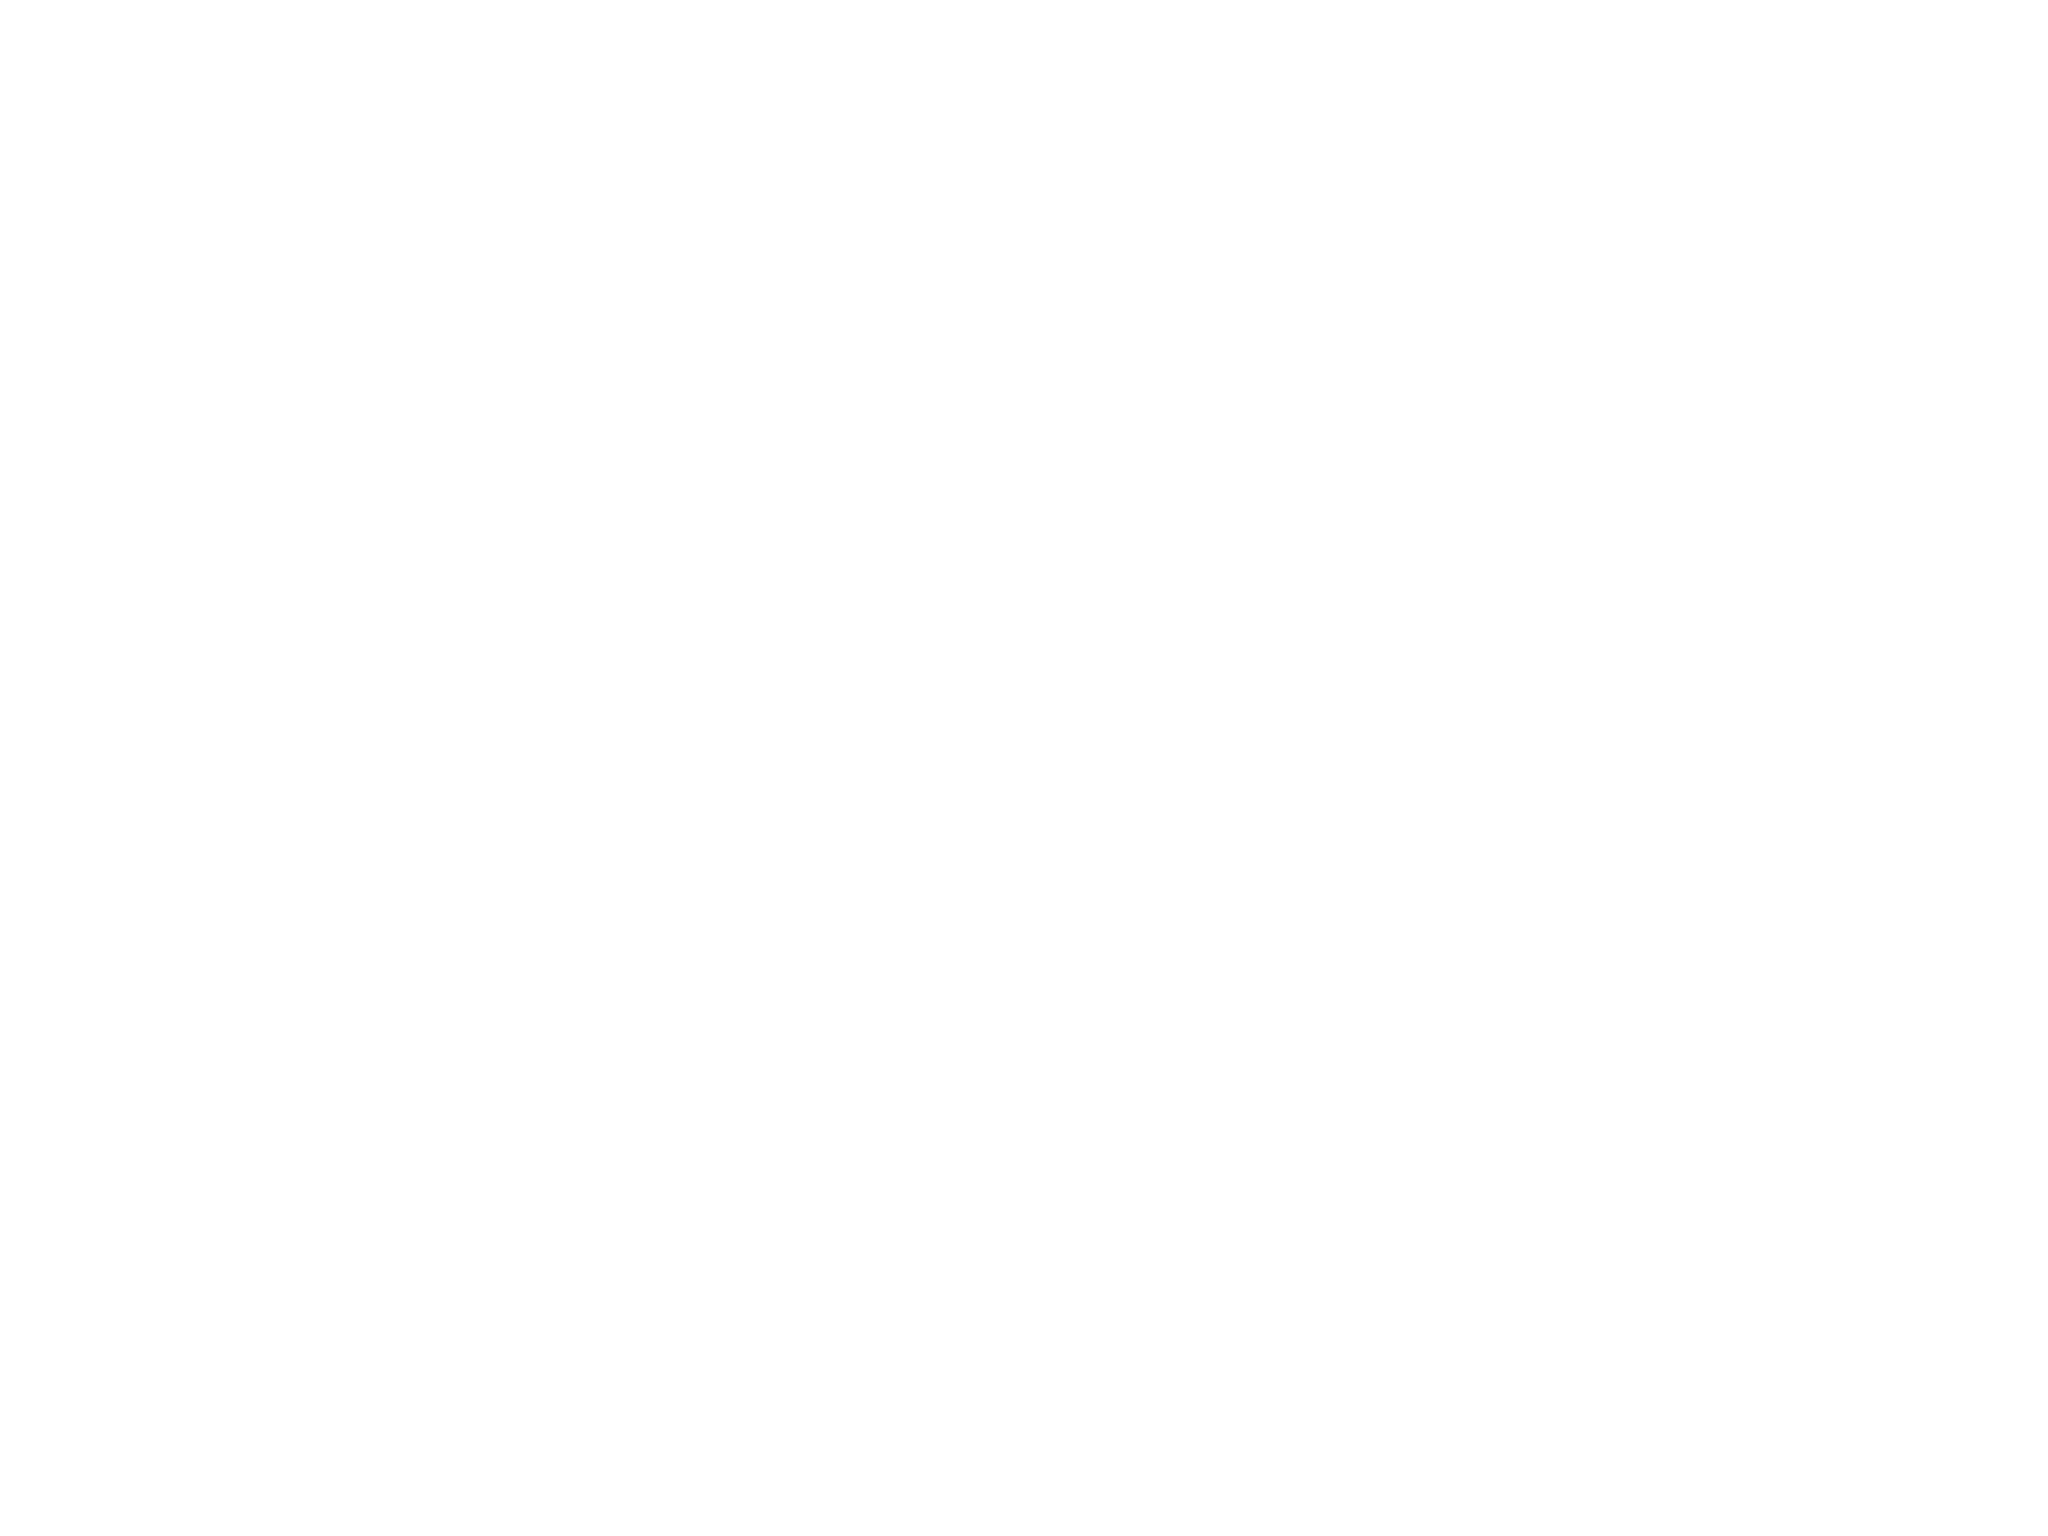
\includegraphics[width=0.85\textwidth]{cpu-beq.pdf}

\end{frame}


\begin{frame}
\frametitle{Rychlost CPU}

\bigskip

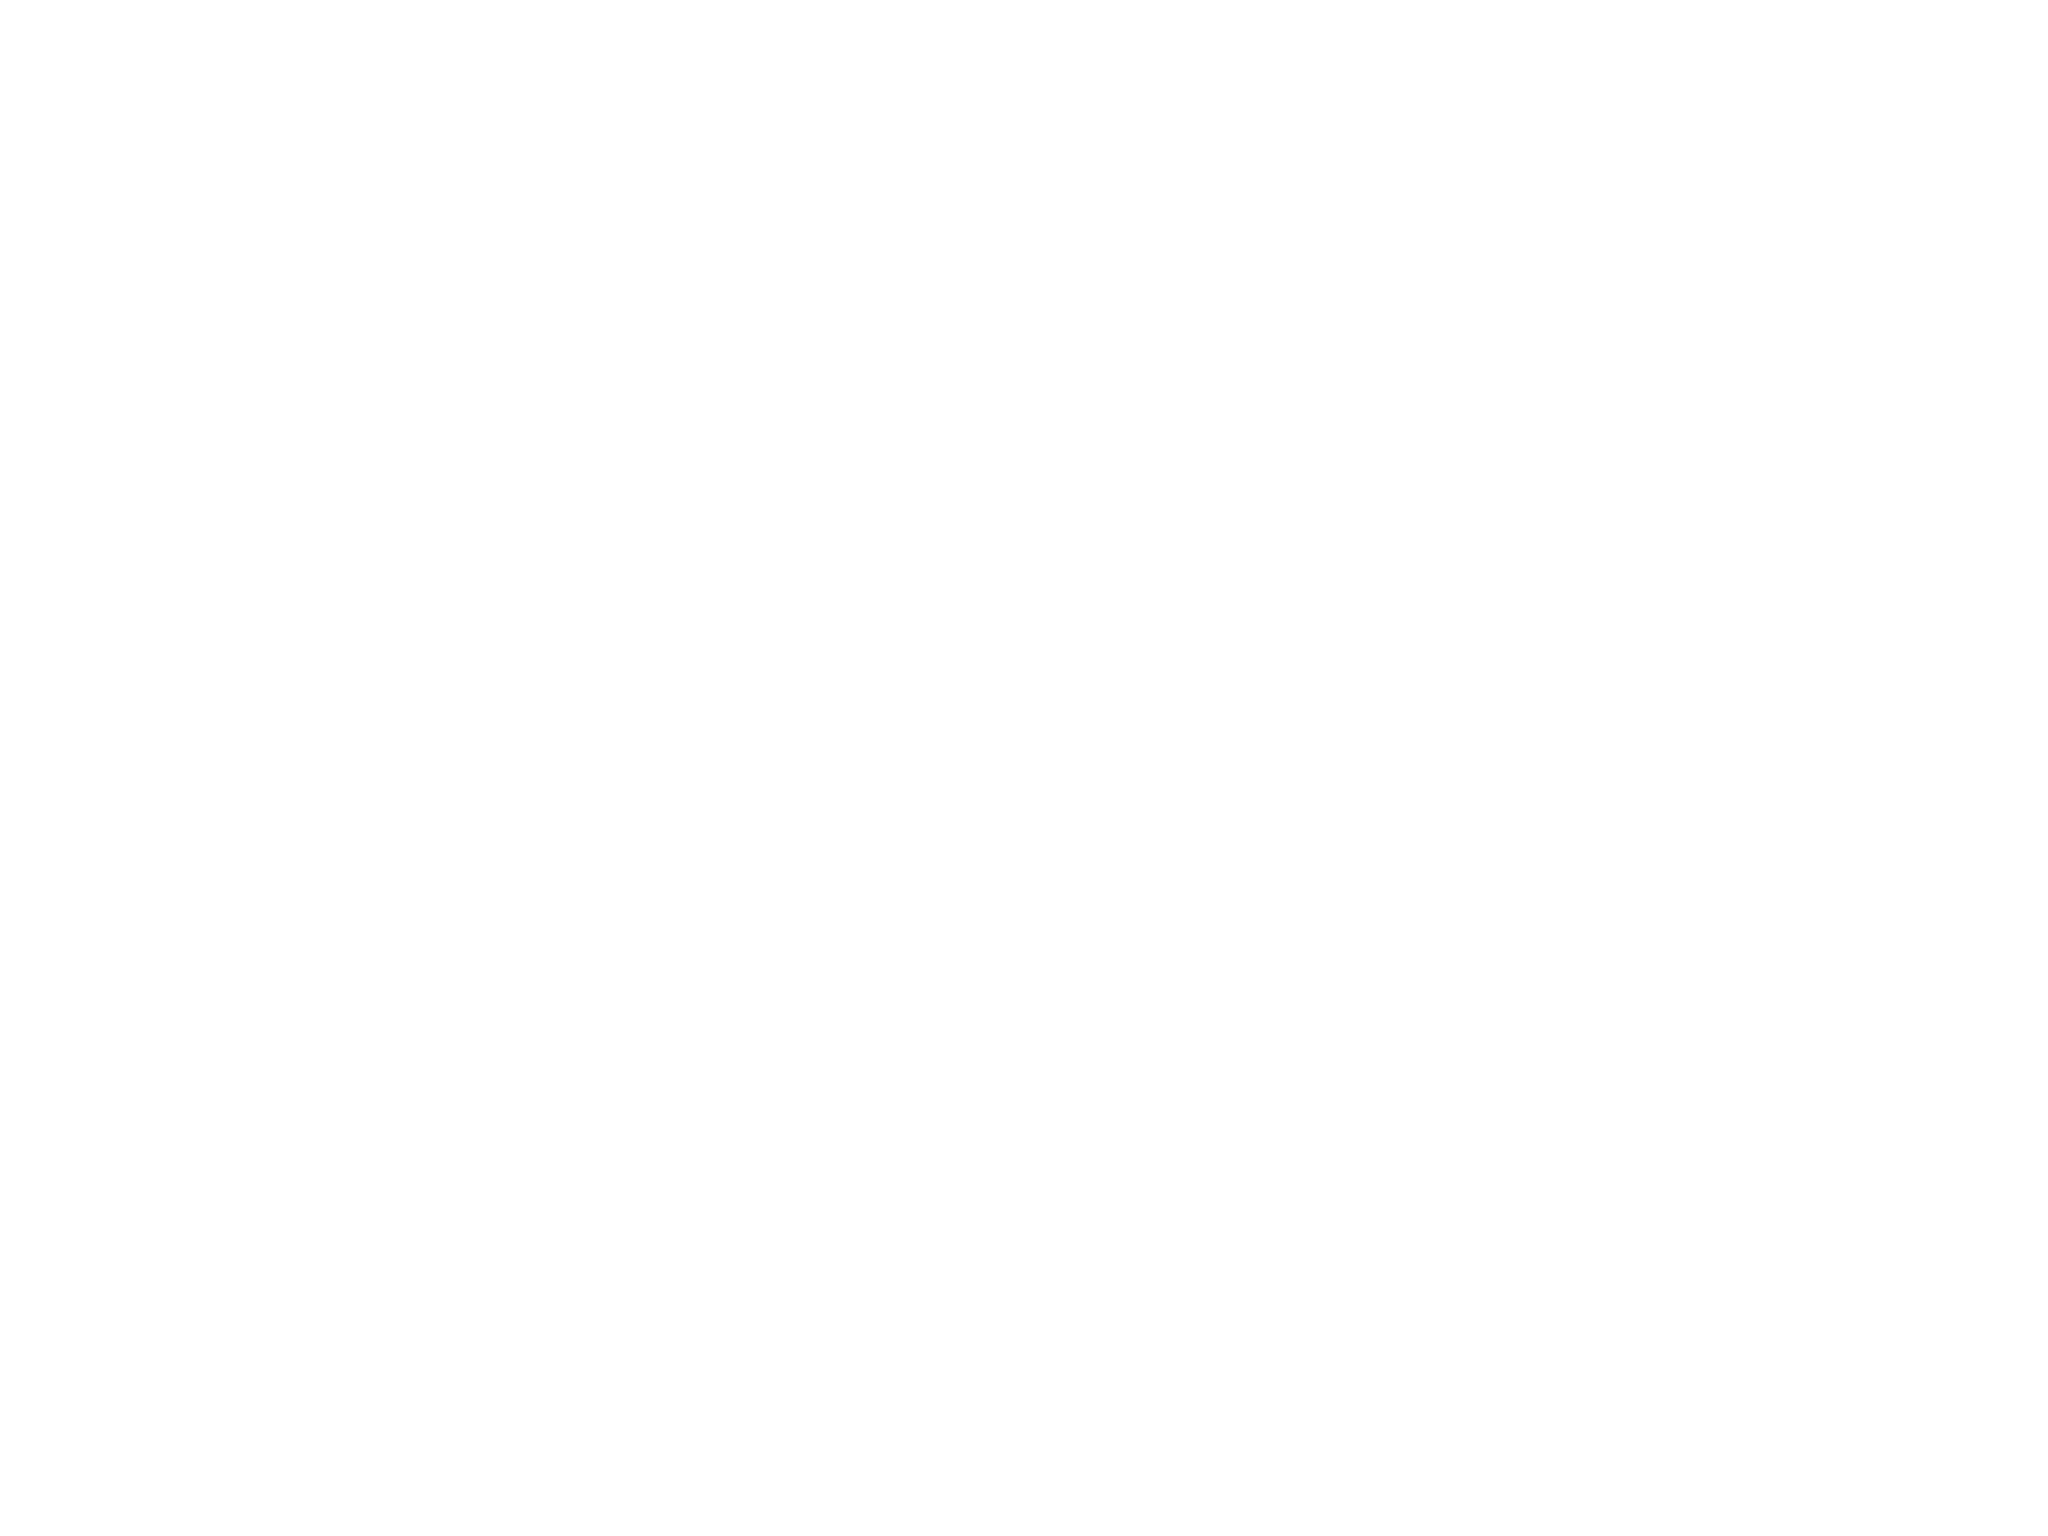
\includegraphics[width=0.85\textwidth]{cpu-time.pdf}

\end{frame}


\begin{frame}
\frametitle{Control Unit}

\bigskip

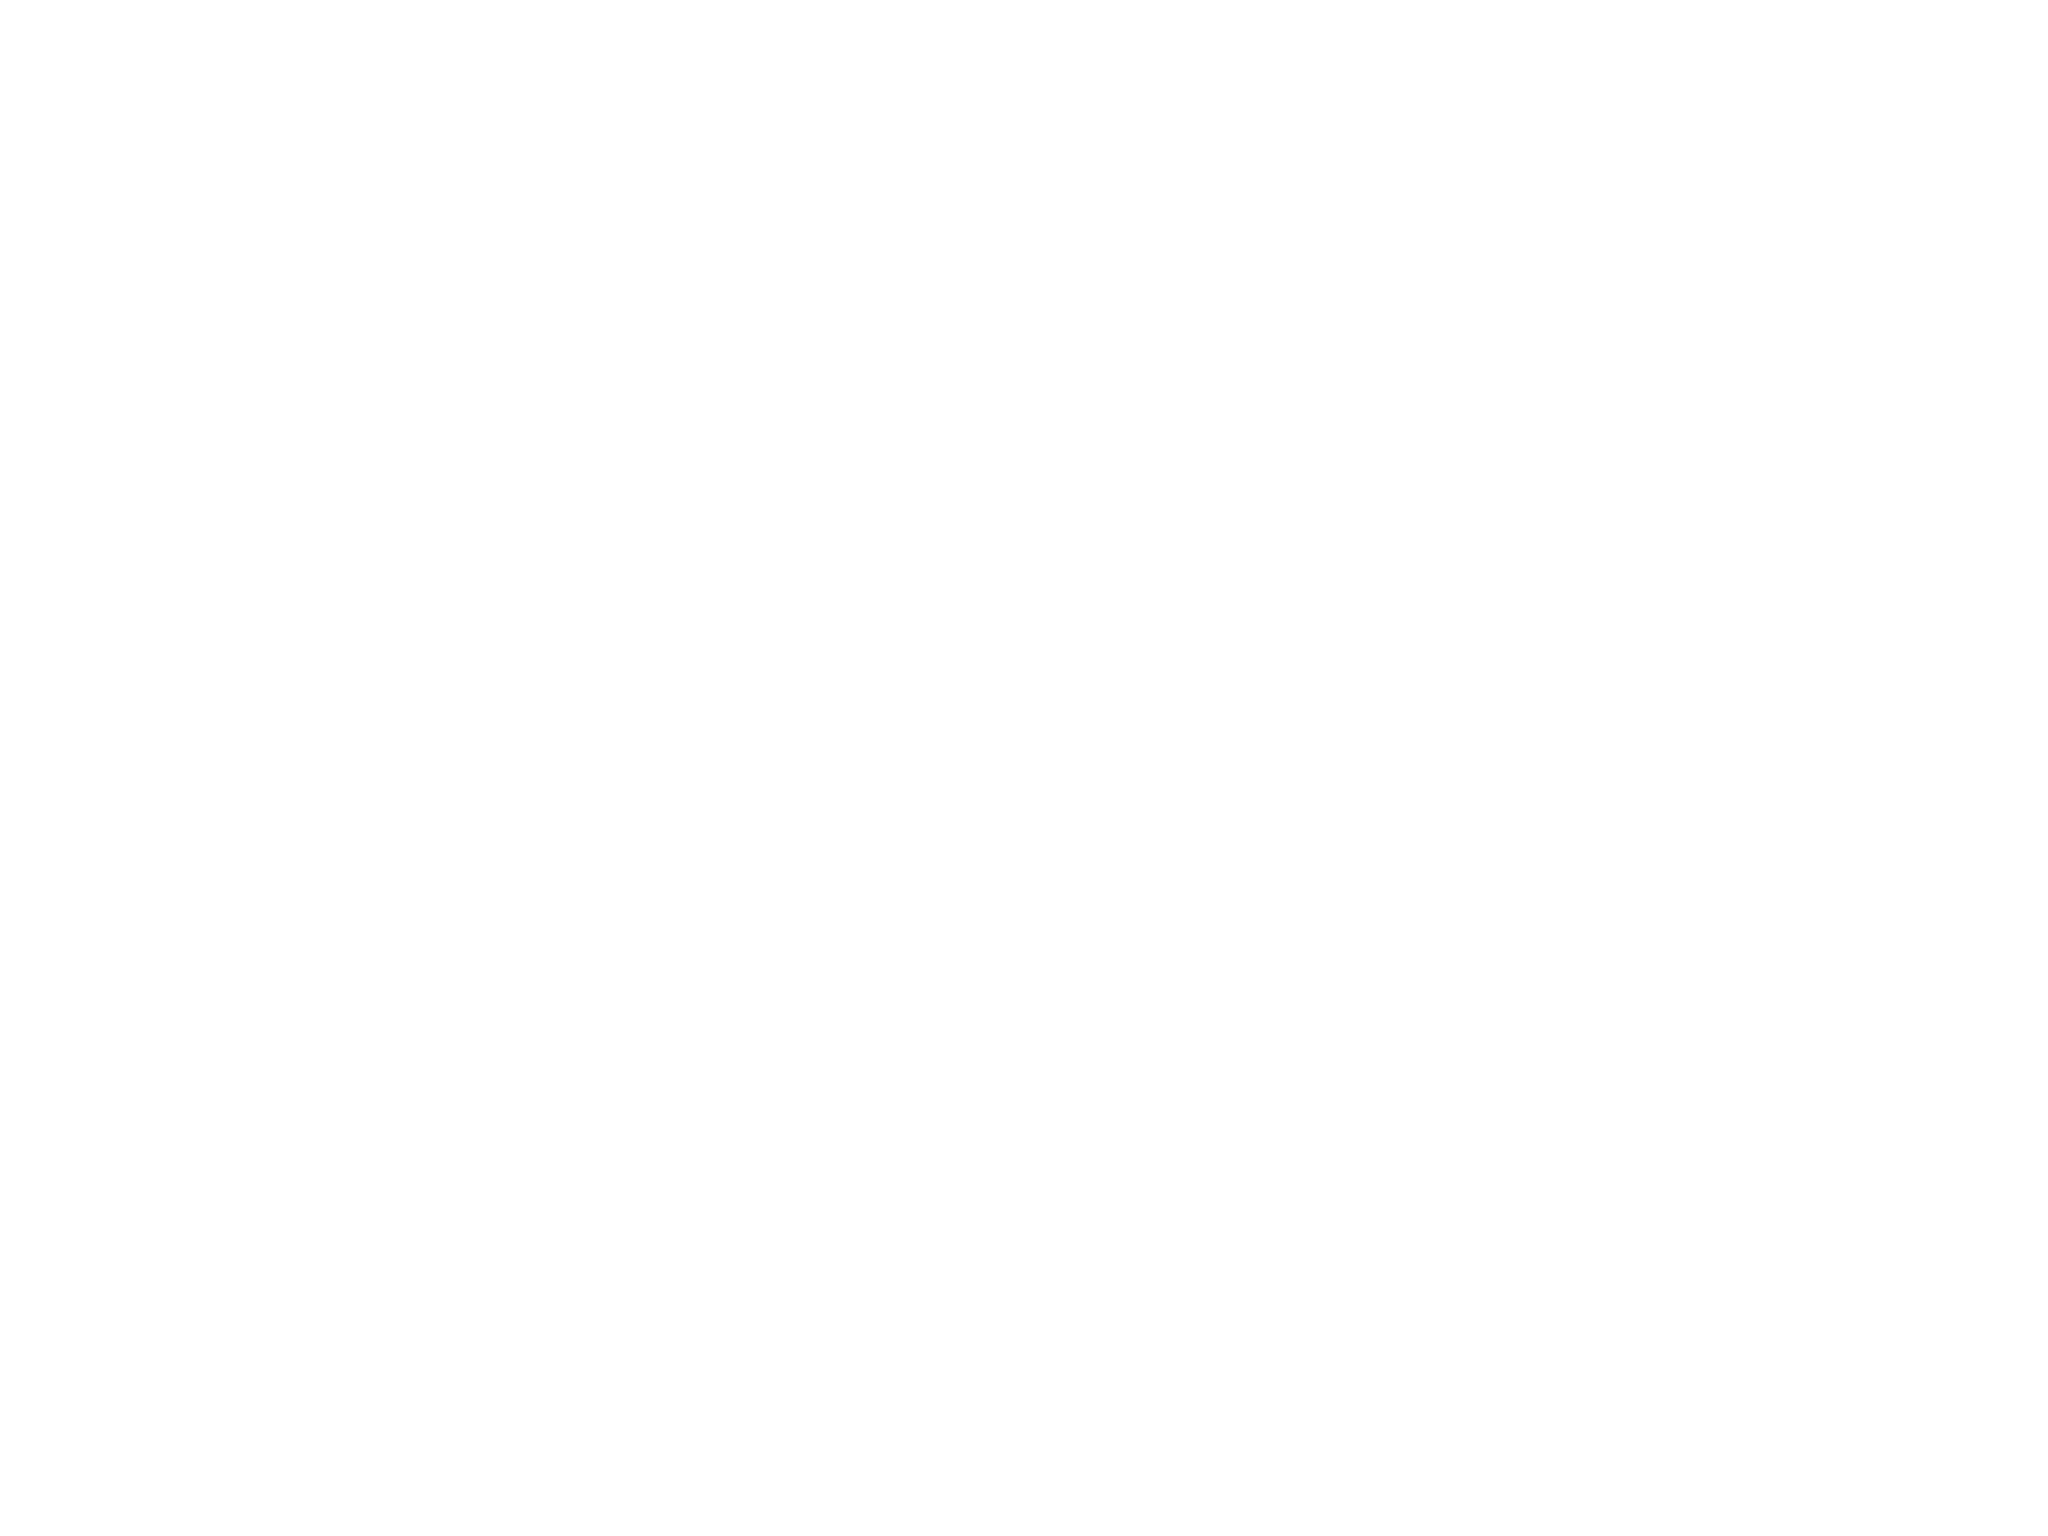
\includegraphics[width=0.85\textwidth]{cpu-control-unit.pdf}

\end{frame}


\end{document}

